\documentclass{article}

\pdfoutput=1
% if you need to pass options to natbib, use, e.g.:
    % \PassOptionsToPackage{numbers, compress}{natbib}
% before loading neurips_2024
\PassOptionsToPackage{numbers, compress}{natbib}

% ready for submission
% \usepackage{neurips_2024}


% to compile a preprint version, e.g., for submission to arXiv, add add the
% [preprint] option:
% \usepackage[preprint]{neurips_2024}


% to compile a camera-ready version, add the [final] option, e.g.:
\usepackage[final]{neurips_2024}


% to avoid loading the natbib package, add option nonatbib:
%    \usepackage[nonatbib]{neurips_2024}


\usepackage[utf8]{inputenc} % allow utf-8 input
\usepackage[T1]{fontenc}    % use 8-bit T1 fonts
% \usepackage{hyperref}       % hyperlinks
\usepackage[colorlinks,
            linkcolor=red,
            anchorcolor=green,
            citecolor=blue
            ]{hyperref} 
\usepackage{url}            % simple URL typesetting
\usepackage{booktabs}       % professional-quality tables
\usepackage{amsfonts}       % blackboard math symbols
\usepackage{nicefrac}       % compact symbols for 1/2, etc.
\usepackage{microtype}      % microtypography
\usepackage{xcolor}         % colors
\usepackage{natbib}
\usepackage{amsmath}
\usepackage{graphicx}
\usepackage{caption}
\usepackage{subcaption} % 用于子图标题
\usepackage{enumitem} % 用于子图标题
\usepackage{wrapfig}
\usepackage{algorithm}
\usepackage{algorithmic}
\usepackage{multirow}
\newcommand{\ie}{\emph{i.e., }}
\newcommand{\eg}{\emph{e.g., }}
\newcommand{\etal}{\emph{et al. }}
\newcommand{\st}{\emph{s.t. }}
\newcommand{\etc}{\emph{etc.}}
\newcommand{\wrt}{\emph{w.r.t. }}
\newcommand{\cf}{\emph{cf. }}
\newcommand{\aka}{\emph{a.k.a. }}
\DeclareMathOperator*{\argmax}{arg\,max}
\DeclareMathOperator*{\argmin}{arg\,min}
\newcommand{\piref}{\pi_\text{ref}}
\newcommand{\pisft}{\pi^\text{SFT}} %
\newcommand{\wb}{\mathbf{w}}
\newcommand{\xb}{\mathbf{x}}
\newcommand{\yb}{\mathbf{y}}
\newcommand{\cX}{\mathcal{X}}
\newcommand{\EE}{\mathbb{E}}
\newcommand{\Set}[1]{\mathcal{#1}}
\definecolor{-}{rgb}{0.25,0.41,0.88}
\definecolor{+}{rgb}{0.70,0.13,0.13}
\newcommand{\wjc}[1]{{{#1}}}
\RequirePackage{bm}
\newcommand{\btheta}{\bm{\theta}}
\title{A Novel Approach to Direct Preference Optimization: Dynamic $\beta$ and Quality-Aware Data Filtering}
\title{$\beta$-DPO: Direct Preference Optimization \\ with Dynamic $\beta$}


% The \author macro works with any number of authors. There are two commands
% used to separate the names and addresses of multiple authors: \And and \AND.
%
% Using \And between authors leaves it to LaTeX to determine where to break the
% lines. Using \AND forces a line break at that point. So, if LaTeX puts 3 of 4
% authors names on the first line, and the last on the second line, try using
% \AND instead of \And before the third author name.

\author{
   Junkang Wu$^{1}$\thanks{Work done at Alibaba Group.}~~Yuexiang Xie$^{2}$~~Zhengyi Yang$^{1}$~~Jiancan Wu$^{1}$\thanks{Jiancan Wu and Xiangnan He are the corresponding authors.}
   ~~\\
   \textbf{Jinyang Gao$^{2}$~~Bolin Ding$^{2}$~~Xiang Wang$^{1}$~~Xiangnan He$^{1}$\footnotemark[2]}\\
  $^{1}$University of Science and Technology of China\\
  $^{2}$Alibaba Group \\
  \texttt{\{jkwu0909, yangzhy1998, wujcan, xiangwang1223, xiangnanhe\}@gmail.com},\\ 
  \texttt{\{yuexiang.xyx, jinyang.gjy, bolin.ding\}@alibaba-inc.com}
}
% \author{%
%   David S.~Hippocampus\thanks{Use footnote for providing further information
%     about author (webpage, alternative address)---\emph{not} for acknowledging
%     funding agencies.} \\
%   Department of Computer Science\\
%   Cranberry-Lemon University\\
%   Pittsburgh, PA 15213 \\
%   \texttt{hippo@cs.cranberry-lemon.edu} \\
%   % examples of more authors
%   % \And
%   % Coauthor \\
%   % Affiliation \\
%   % Address \\
%   % \texttt{email} \\
%   % \AND
%   % Coauthor \\
%   % Affiliation \\
%   % Address \\
%   % \texttt{email} \\
%   % \And
%   % Coauthor \\
%   % Affiliation \\
%   % Address \\
%   % \texttt{email} \\
%   % \And
%   % Coauthor \\
%   % Affiliation \\
%   % Address \\
%   % \texttt{email} \\
% }


\begin{document}


\maketitle


\begin{abstract}
Direct Preference Optimization (DPO) has emerged as a compelling approach for training Large Language Models (LLMs) to adhere to human preferences. However, the performance of DPO is sensitive to the fine-tuning of its trade-off parameter $\beta$, as well as to the quality of the preference data. We analyze the impact of $\beta$ and data quality on DPO, uncovering that optimal $\beta$ values vary with the informativeness of pairwise data. Addressing the limitations of static $\beta$ values, we introduce a novel framework that dynamically calibrates $\beta$ at the batch level, informed by data quality considerations. Additionally, our method incorporates $\beta$-guided data filtering to safeguard against the influence of outliers. Through empirical evaluation, we demonstrate that our dynamic $\beta$ adjustment technique significantly improves DPO's performance across a range of models and datasets, offering a more robust and adaptable training paradigm for aligning LLMs with human feedback. The code is available at \url{https://github.com/junkangwu/beta-DPO}.
\end{abstract}

\section{Introduction}
\label{Introduction}
The alignment of Large Language Models (LLMs) with human feedback, as explored in works like GPT-4 and LLaMA-2 \cite{GPT4,llama2,GPT4_2}, has marked a significant advancement in generating responses that are more helpful, factual, and ethical \cite{instructGPT}. Among the various alignment strategies, Reinforcement Learning from Human Feedback (RLHF) \cite{instructGPT} is a notable method that refines LLMs using the Proximal Policy Optimization (PPO) algorithm \cite{PPO}. This approach employs a KL divergence penalty to ensure minimal deviation of the model from its original configuration, ensuring the retention of its initial characteristics while improving alignment.

Despite the effectiveness, RLHF's instability and computational requirements often limit its practical applications, prompting the exploration of alternatives like Direct Preference Optimization (DPO) \cite{DPO}. DPO circumvents the reinforcement learning loop by exploiting the inherent connection between reward functions and optimal policies, thereby simplifying the policy model training. It encourages the model to favor the response that aligns with human preferences ($\yb_{w}$) over the dispreferred ($\yb_{l}$), \wjc{implying DPO's sensitivity to the quality of pairwise data}. 
The balance between maintaining the original reference model ($\pi_{\text{ref}}$) and incorporating new preferences ($\pi_{\btheta}$) is controlled by a $\beta$ hyperparameter, whose lower values advocate for aggressive updates and higher values support more conservative adjustments:
\begin{align*}
    \ell_{\text{DPO}}(\btheta)=\EE_{\xb,\yb_{w},\yb_{l}} [-\log \sigma \big(
    \beta \big[
    \log \big(\frac{\pi_{\btheta}(\yb_{w}|\xb)}{\pi_{\text{ref}}(\yb_{w}|\xb)}\big)
    -
    \log \big(\frac{\pi_{\btheta}(\yb_{l}|\xb)}{\pi_{\text{ref}}(\yb_{l}|\xb)}\big)
    \big]
    \big)].
\end{align*}
However, the current DPO literature has largely overlooked the joint influence of $\beta$ selection and pairwise data $(\yb_{w}, \yb_{l})$'s quality on the alignment performance.
\wjc{To bridge this gap, we conduct a preliminary experiment to investigate how different $\beta$ selections influence the model performance under two distinct data pair gap conditions, as shown in Figure \ref{fig_1_2}.}
In \emph{low gap} scenarios (\cf Figure \ref{fig_1_1}),
where the difference between preferred and dispreferred samples is minor, an increase in $\beta$ (\eg from 0.1 to 0.5) corresponds with a decline in win rate (\eg from 42\% to 33\%).
Conversely, in \emph{high gap} situations (\cf Figure \ref{fig_1_1})
where a significant difference exists, an increase in $\beta$ tends to improve DPO performance.
\wjc{Such contrasting outcomes highlight the necessity to tailor the $\beta$ value contingent upon the data quality, especially in the presence of outliers \cite{outlier_dataset}.}
\begin{figure}
    \centering
    \begin{subfigure}{.65\textwidth}
      \centering
      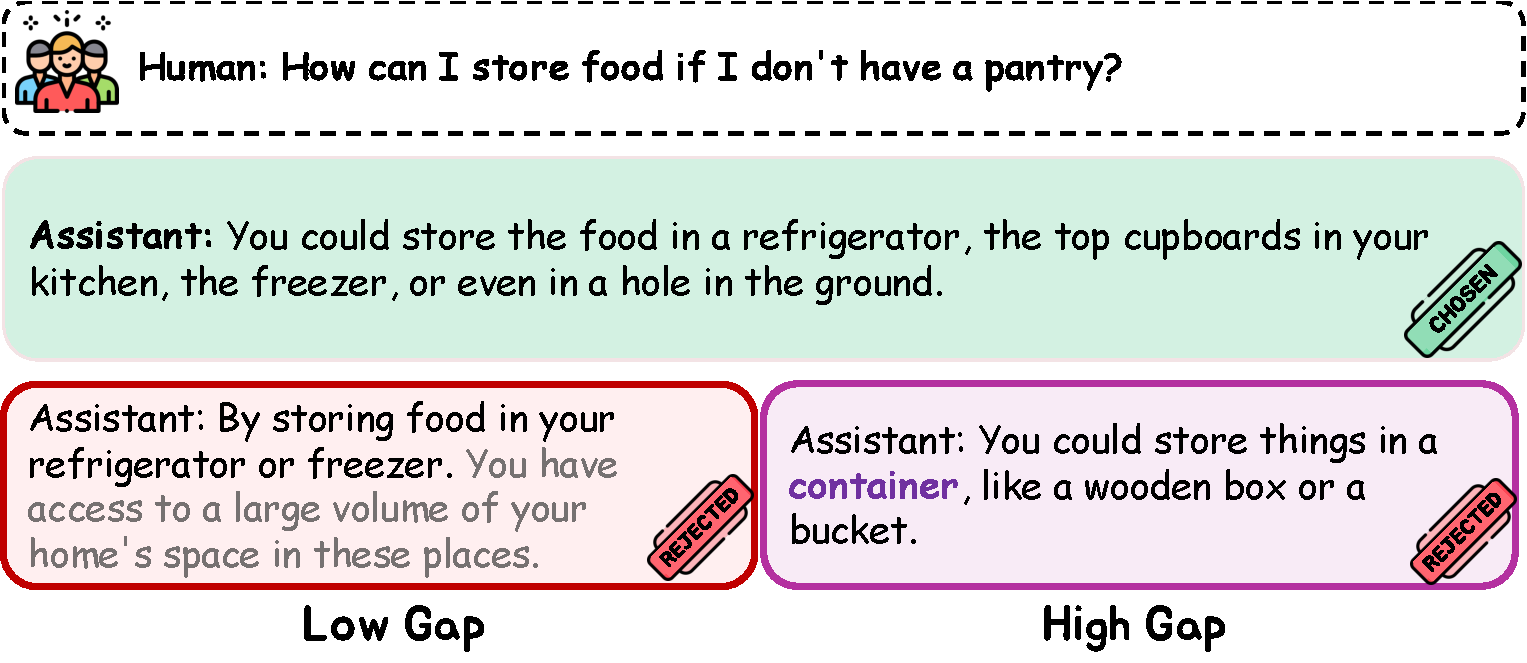
\includegraphics[width=\linewidth]{figs/first_fig_a.pdf}
      \caption{} % 你可以在这里添加子图标题
      \label{fig_1_1}
    \end{subfigure}%
    \hfill % 这会在子图之间添加一些空间
    \begin{subfigure}{.3\textwidth}
      \centering
      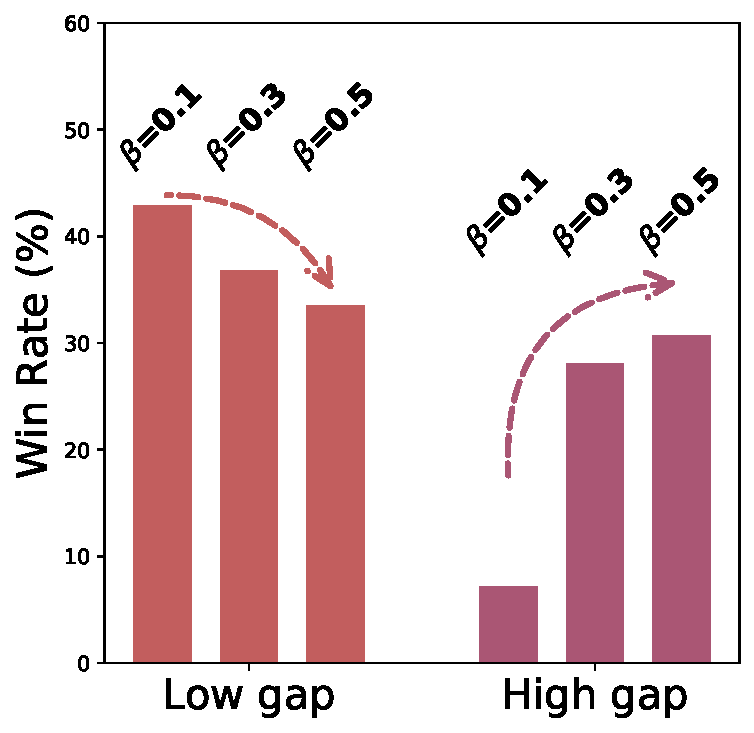
\includegraphics[width=\linewidth]{figs/NeurIPS_first_fig.pdf}
      \caption{} % 同样,为第二个子图添加标题
      \label{fig_1_2}
    \end{subfigure}
    \caption{
    \textbf{(\ref{fig_1_1}) Pairwise Data: Low vs. High Gap}: ``Low gap'' denotes cases where the chosen and rejected examples are closely similar, typically indicating high-quality, informative pairs. ``High gap'' signifies pairs with larger differences, implying lower-quality data.
    \textbf{(\ref{fig_1_2}) Influence of Data Quality on $\beta$ Selection:} Pythia-1.4B's performance on the HH dataset reveals a distinct trend: for ``Low gap'', a higher $\beta$ reduces win rate, whereas for ``High gap'', an increased $\beta$ improves it.}
    \label{fig:combined}
\end{figure}

Building upon these insights and recognizing the mixture nature of diverse quality in practically collected data \cite{mixture_data},
we propose a dynamic $\beta$ selection strategy for DPO. This strategy adaptively adjusts $\beta$ in response to the quality of pairwise data and robustifies DPO against data variability. 
Intuitively, one straightforward solution is personalizing $\beta$ for each pair, rather than fixing it across the population of all pairs. While conceptually appealing, (1) instance-level $\beta$ personalization can lead to optimization instabilities, particularly when dealing with a vast array of human preference instances \wjc{(\cf Section \ref{sec_batch_level})}. This issue underscores the challenge of balancing $\beta$ updates with stable and scalable DPO. In this light, we propose to explore a \textit{batch-level} adaptation of $\beta$, aiming to balance update aggressiveness and training stability. Moreover, (2) the frequent occurrence of outliers necessitates a strategy for accurately adjusting the batch-level $\beta$. 
The dataset notably features outliers, a challenge underscored by the significant reward discrepancy variations within the training samples of the dataset (\cf Section \ref{motivation_sec}). 
Such conditions impede the model's ability to accurately estimate the batch-level $\beta$, thereby undermining the effectiveness of batch-level $\beta$ calibration.
To this end, we propose a simple yet effective dual-component approach:


\begin{itemize}[leftmargin=*]
  \item \textbf{Dynamic $\beta$ Calibration at Batch-Level} (for Challenge 1): To mitigate optimization instabilities, we dynamically calibrate $\beta$ within each batch. Specifically, this batch-level adjustment is based on data quality, with $\beta$ being adaptively decreased for high-quality, closely-matched pairwise data (\ie \emph{low gap} data) to facilitate assertive updates. While for easily-discriminated pairs (\ie \emph{high-gap} data), $\beta$ is increased to promote cautious updates, preventing overfitting to noise.
  This targeted batch-level calibration enables stable and responsive optimization.
  \item \textbf{$\beta$-Guided Data Filtering} (for Challenge 2): We implement a $\beta$-guided data filtering approach to tackle the frequent occurrence of outliers. By establishing a benchmark $\beta$ value for filtering incoming data at the batch level, we maintain the fidelity of $\beta$ estimation by prioritizing the most reliable and representative samples. As a result, it diminishes the impact of outliers that might otherwise derail the optimization process, thus enhancing the precision and robustness of the batch-level $\beta$ calibration.
\end{itemize}

Our contributions are threefold: (1) We investigate a pioneering study on the joint influence of $\beta$ selection and pairwise data quality on the DPO performance. (2) We introduce a simple yet effective $\beta$-dynamic strategy for DPO, adaptively balancing the update aggressiveness and training stability. (3) Through empirical evaluations, our approach demonstrates marked improvements in performance across diverse conditions and model sizes
(\eg achieving improvements exceeding 10\% on models of various sizes, including Pythia-410M, 1.4B, and 2.8B).

% To navigate these challenges, our research introduces a dual-optimization strategy: first, dynamically adjusting $\beta$ at the batch level according to the data quality and second, employing a filtration mechanism that leverages a benchmarked $\beta$ to reduce outlier interference. We pioneer in unraveling the relation between $\beta$ parameters and pairwise data quality, suggesting an innovative and adaptable solution. Our empirical validation across diverse settings and model sizes confirms that this dynamic $\beta$ strategy enhances performance significantly.

% Our contributions are threefold: (1) We present a pioneering study on how the quality of pairwise data influences the choice of $\beta$. (2) We introduce a novel dynamic $\beta$ mechanism, responsive to data quality. (3) Through empirical evaluations, our approach demonstrates marked improvements in performance across diverse conditions and model sizes.

% This paper proposes a dynamic approach to the $\beta$ parameter in DPO, aiming to adapt to a diverse range of preference data. We identify two principal challenges in implementing dynamic $\beta$: the risk of unstable optimization when assigning unique $\beta$ values to individual data instances, and the influence of outliers when determining batch-level $\beta$ settings. To innovate within these constraints, we devise a dual optimization strategy:


% \textbf{Dynamic $\beta$ Calibration with Batch-Level Adaptation:} This mechanism dynamically calibrates the $\beta$ value in response to the quality of pairwise preference data. By evaluating the proximity between preferred responses and their references, $\beta$ is decreased to encourage more assertive updates when the data indicates a close match and high quality (\emph{low gap}). Conversely, in cases where the data exhibits a \emph{High gap}, $\beta$ is increased to endorse more conservative updates, safeguarding against potential overfitting to noisy or less informative data.

% \textbf{$\beta$-Guided Data Filtering:} To enhance the accuracy of $\beta$ calibration and mitigate the effects of outliers, we implement a selective data filtering process. This method utilizes a benchmark $\beta$ value to screen the incoming data at the batch level, ensuring that the estimation of $\beta$ is based on the most reliable and representative samples. Consequently, this assists in reducing the influence of outliers that could otherwise skew the optimization trajectory.

% \textbf{Beta Quality Adjustment:} The $\beta$ value adjusts based on the proximity between preferred responses and references, promoting more vigorous updates in scenarios with close-mapped high-quality data (Low Gap) and maintaining cautious updates in the presence of broader gaps (High Gap).

% \textbf{Data Filtering:} A filtering process is employed to refine the influence of outliers on $\beta$ estimation at the batch level.



% Our empirical inquiry reveals the nuanced influence of (\beta)'s magnitude on DPO's generative performance. As depicted in Figure \ref{fig_1_2} (red bars), altering (\beta) from 0.1 to 0.5 correlates with a reduction in win rate, declining notably from 42\% to 33\%—a testament to the delicate interplay between hyperparameter tuning and model output. This sensitivity is further modulated by the quality of training pairs, a factor we corroborate quantitatively. Data pairs exhibiting a \emph{low gap} generally convey a high informational content, fostering a setting where a reduced (\beta) bolsters effective policy learning. In stark contrast, when confronted with a \emph{high gap}, indicative of sparse information, a conservative (\beta) is prudent to avoid overfitting trivial discrepancies. The optimal calibration of (\beta) thus navigates a spectrum conditioned by data quality differentiation, as evidenced by our comparison between different gap levels (purple bars in Figure \ref{fig_1_2}). The shifting landscape of (\beta) efficacy, especially in settings rife with outliers, underscores the inadequacy of static (\beta) application within the DPO framework.

% Our investigations reveal that the performance of DPO is intricately linked with the selection of the $\beta$ parameter and the quality of the training pairs. Notably, typical practice often defaults $\beta$ to a static value, for instance, 0.1. However, as our empirical findings depict in Figure \ref{fig_1_2} (red bars), such a one-size-fits-all approach may not be ideal. The generative capacity of DPO showcased marked variations with adjustments in $\beta$; an increase from 0.1 to 0.5 led to a pronounced drop in the win rate, plummeting from 42\% to 33\%. This sensitivity is further complicated by the inherent quality of the data, where we witness the optimal selection of (\beta) shifting in response to the nature of the training pairs evaluated. The low gap versus high gap comparison elucidates this dynamic, with optimum $\beta$ values diverging under different data quality scenarios, as illustrated by the purple bars in Figure \ref{fig_1_2}.

% This empirically informed perspective underscores a critical observation — statically fixed (\beta) values are suboptimal for DPO in real-world scenarios marred by data variability and outliers. For example, training pairs closely aligned (\emph{low gap}) are rich in informative content, demanding a lower (\beta) to facilitate effective policy updates. Conversely, pairs with significant dissimilarities (\emph{high gap}) prompt a higher (\beta), mitigating the risk of overfitting on potentially less informative examples. Such nuanced understanding, enabled by our data-driven analysis, sets the stage for a dynamically adapted (\beta), tailored to the batch-specific characteristics and tackling the variability presented by outliers head on.

% Often, the $\beta$ value is typically set to a fixed value, such as $0.1$. But, the generative performance of DPO exhibits a marked sensitivity to the parameter $\beta$, as illustrated in Figure \ref{fig_1_2} (red bars). Notably, when $\beta$ is increased from 0.1 to 0.5, we observe a decline in the win rate from 42\% to 33\%. And the optimal selection of $\beta$ is subject to shift due to variations in data quality (purple bars in \ref{fig_1_2}). For alignment, informative and high quality pairwise data are intuitively those pairs that are mapped nearby (low gap between $\yb_{w}$ and $\yb_{l}$) but should be far apart. By comparing pairs of ($\yb_{w},\yb_{l}$) at different levels of gap (low gap vs. high gap), it is observed that the optimal value of $\beta$ alters correspondingly. Consequently, given the presence of variability in data quality (i.e., outliers) in real-world scenarios, \emph{a fixed $\beta$ is no longer the optimal choice for the DPO.}

% Empirical evidence suggests that the optimal $\beta$ is sensitive not just to its selection but also to the nature of the training pairs. When too close (\emph{low gap}), the pairs harbor rich information, necessitating a lower $\beta$ for effective policy updates. Conversely, when pairs are evidently disparate (\emph{high gap}), a conservative $\beta$ avoids overfitting on less informative examples. The influence of data variability, especially outliers, becomes significant in real-world distributions, invalidating a static $\beta$ choice.

% Motivated by this, we propose a dynamic selection of $\beta$, which is informed by the quality of pairwise data and addresses data variability robustly. The implementation of this strategy introduces two key challenges: (1) instance-wise $\beta$ attribution can lead to optimization instabilities, and existing population-level approaches do not suffice. Therefore, we propose a batch-level adaptation of $\beta$, balancing update aggressiveness and training stability. (2) The prevalence of outliers necessitates a method to identify and adjust the batch-level $\beta$ appropriately.

% To navigate these challenges, our research introduces a dual-optimization strategy: first, dynamically adjusting $\beta$ at the batch level according to the data quality and second, employing a filtration mechanism that leverages a benchmarked $\beta$ to reduce outlier interference. We pioneer in unraveling the relation between $\beta$ parameters and pairwise data quality, suggesting an innovative and adaptable solution. Our empirical validation across diverse settings and model sizes confirms that this dynamic $\beta$ strategy enhances performance significantly.

% Aligning Large Language Models (LLMs) \cite{GPT4,llama2,GPT4_2} with human feedback has become a critical step to ensure that their outputs are helpful, factual, and ethical \cite{instructGPT}. Despite the effectiveness of Reinforcement Learning from Human Feedback (RLHF) \cite{instructGPT} using the Proximal Policy Optimization (PPO) algorithm \cite{PPO}, it incurs non-negligible costs in terms of stability and computational demand compared to supervised methods. This approach utilizes a reverse KL divergence penalty to guarantee the modeled behavior does not significantly stray from its trained foundation.

% Direct Preference Optimization (DPO) \cite{DPO} has emerged as a promising alternative, streamlining alignment by bypassing complex RL procedures. DPO directly maps preferences, leveraging pairwise comparisons between human-favored responses $\yb_{w}$ and reference responses $\yb_{l}$. The hyperparameter $\beta$ modulates the inclination towards the preferred responses by adjusting the policy model's updates. However, surprisingly, considerations regarding the choice of $\beta$ and the quality of pairwise preference data have been overlooked in existing DPO applications.

% This paper proposes a dynamic approach to the $\beta$ parameter in DPO, aiming to adapt to a diverse range of preference data. We identify two principal challenges in implementing dynamic $\beta$: the risk of unstable optimization when assigning unique $\beta$ values to individual data instances, and the influence of outliers when determining batch-level $\beta$ settings. To innovate within these constraints, we devise a dual optimization strategy:

% \textbf{Beta Quality Adjustment:} The $\beta$ value adjusts based on the proximity between preferred responses and references, promoting more vigorous updates in scenarios with close-mapped high-quality data (Low Gap) and maintaining cautious updates in the presence of broader gaps (High Gap).

% \textbf{Data Filtering:} A filtering process is employed to refine the influence of outliers on $\beta$ estimation at the batch level.

% Our contributions are threefold: (1) We present a pioneering study on how the quality of pairwise data influences the choice of $\beta$. (2) We introduce a novel dynamic $\beta$ mechanism, responsive to data quality. (3) Through empirical evaluations, our approach demonstrates marked improvements in performance across diverse conditions and model sizes.



% DPO relies on two key ingredients: the selection of $\beta$ and the quality of pairwise data. The training objective guides the policy model to prefer the human-preferred action over the reference action by a margin. The $\beta$ value is a hyperparameter that controls the deviation from the base reference policy $\piref$. A smaller $\beta$ value leads to a more aggressive update, while a larger $\beta$ value leads to a more conservative update. 

% The quality of the pairwise data is crucial for the model to learn effectively. In the context of DPO, the quality of the pairwise data is assessed by the reward differences between the sample pairs. When the pairwise data is of high quality, a small and fixed $\beta$ is sufficient to achieve good performance. However, when the pairwise data is of poor quality or not all high quality, the small and fixed $\beta$ will lead to overfitting.


% Therefore, the methodology advanced here is keenly attuned to outlier detection and management, ensuring the integrity of the batch-optimized beta determination.

% To 
% In this work, we employ a \textit{danamic} $\beta$ during training and 
% And the pairwise data are assumed to be of high quality. 

% However, the optimal $\beta$ value is contingent upon the quality of the pairwise data. When the pairwise data is of high quality, a small and fixed $\beta$ is sufficient to achieve good performance. However, when the pairwise data is of poor quality or not all high quality, the small and fixed $\beta$ will lead to overfitting. In this paper, we propose a method to estimate a better $\beta$ that upholds Principle 1, and simultaneously combines this idea with data filtering to address Principle 2.
% leverages the mapping between the reward
% function and the optimal policy to bypass the need for reinforcement learning and explicit reward
% model learning.
% has emerged as an alternative

% Despite the DPO has exhibited exceptional performance across a variety of tasks, we remain intrigued by the potential to maximize the capabilities of DPO. To this end, our inquiry is particularly focused on two aspects: the selection of the $\beta$ and the quality of pairwise data. As illustrated in Figure 1(a) through validation experiments conducted on the HH dataset, it becomes evident that 1) the generative performance of the model exhibits a marked sensitivity to the parameter $\beta$. Notably, when $\beta$ is increased from 0.1 to 0.5, we observe a decline in the win rate from 42\% to 33\%. 
% Simultaneously, 2) the optimal selection of $\beta$ is subject to shift due to variations in data quality. As demonstrated by the purple bars in Figure 1, we substitute the negative samples with those generated by the supervised fine-tuning (SFT) model (high gap). By comparing pairs of positive and negative samples at different levels of difficulty (low gap vs. high gap), it is observed that the optimal value of $\beta$ alters correspondingly. 

% Consequently, we posit that the DPO encounters a complex challenge in discerning distinctions between samples of varying quality levels. 

% This observation underscores the imperative of refining our approach to data quality and parameter optimization to fully leverage the potential of DPO in handling diverse and challenging datasets.

% Despite the DPO has exhibited exceptional performance across a variety of tasks, we remain intrigued by the potential to maximize the capabilities of DPO. To this end, our inquiry is particularly focused on two aspects: the selection of the $\beta$ and the quality of pairwise data. As depicted in Figure 1(a) through validation on the HH dataset, it becomes evident that the choice of $\beta$ values exerts a significant impact on the model's performance.Notably, when $\beta$ is increased from 0.1 to 0.5, we observe a decline in the win rate from 42\% to 33\%.

%  notably, $\beta$ increased from 0.1 to 0.5, the win rate 由42\%下降到33\%., . Furthermore, as demonstrated in Figure 1(b), the optimal selection of $\beta$ is also contingent upon the quality of data. By constructing positive and negative sample pairs of varying levels, we observe a proportional increase in the optimal $\beta$ value as the reward difference between the sample pairs increases. This phenomenon leads us to speculate on the influence of outliers in this context.

% Despite the DPO has exhibited exceptional performance across a variety of tasks, we remain intrigued by the potential to maximize the capabilities of DPO. To this end, our inquiry is particularly focused on two aspects: the selection of the $\beta$ and the quality of pairwise data. As depicted in Figure 1(a) through validation on the IMDB dataset, it is clear that different $\beta$ values significantly influence model performance; notably, an excessively large $\beta$ impedes model updates, thereby adversely affecting performance metrics. Furthermore, as demonstrated in Figure 1(b), the optimal selection of $\beta$ is also contingent upon the quality of data. By constructing positive and negative sample pairs of varying levels, we observe a proportional increase in the optimal $\beta$ value as the reward difference between the sample pairs increases. This phenomenon leads us to speculate on the influence of outliers in this context.
% \begin{figure}
%     \centering
%     \begin{subfigure}{.65\textwidth}
%       \centering
%       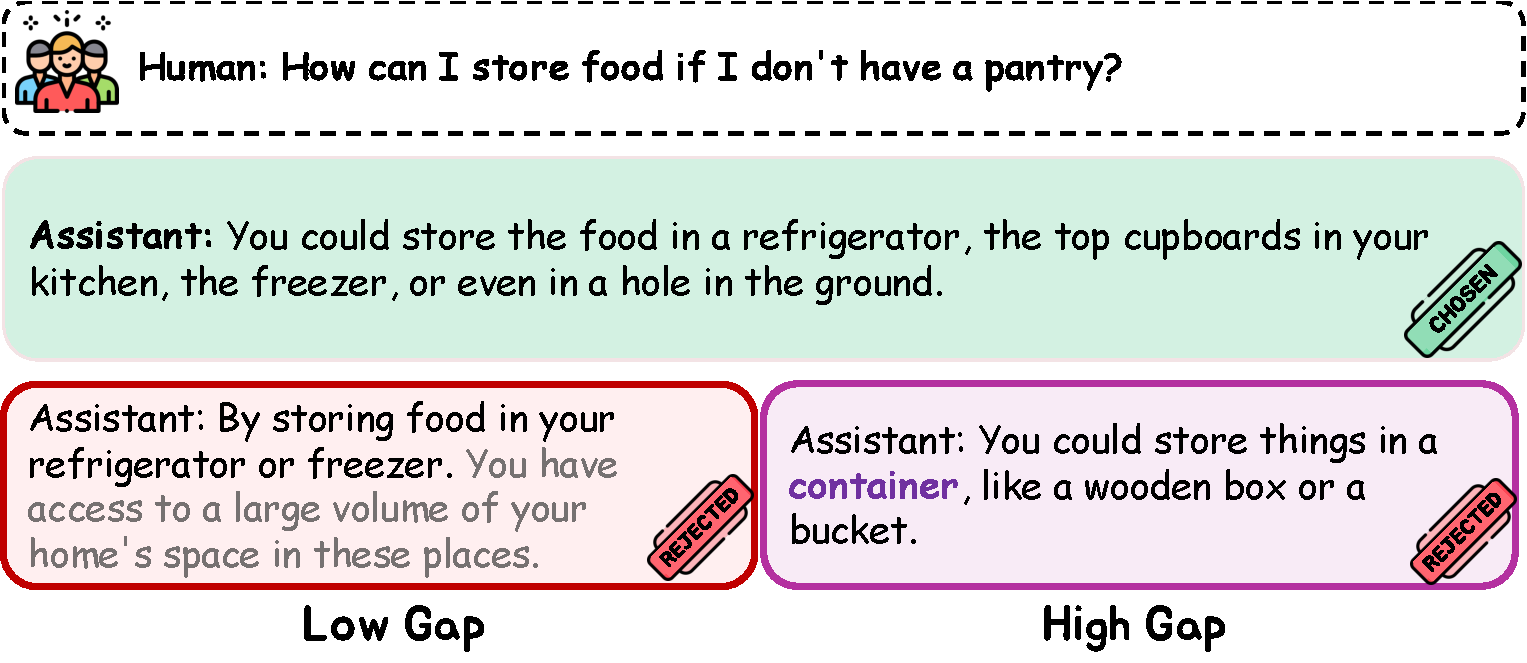
\includegraphics[width=\linewidth]{figs/first_fig_a.pdf}
%       \caption{} % 你可以在这里添加子图标题
%       \label{fig_1_1}
%     \end{subfigure}%
%     \hfill % 这会在子图之间添加一些空间
%     \begin{subfigure}{.3\textwidth}
%       \centering
%       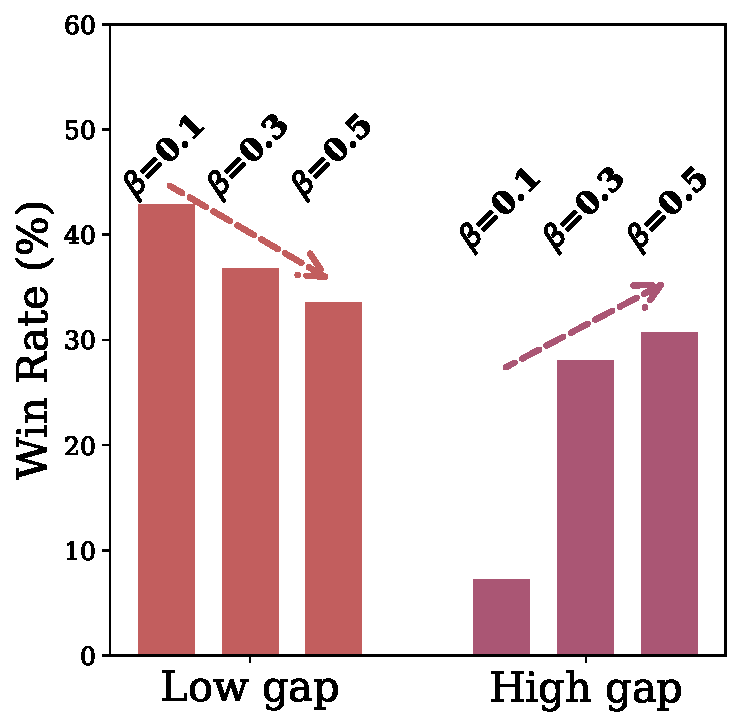
\includegraphics[width=\linewidth]{figs/first_fig.pdf}
%       \caption{} % 同样,为第二个子图添加标题
%       \label{fig_1_2}
%     \end{subfigure}
%     \caption{
%     \textbf{(\ref{fig_1_1}) Pairwise Data: Low vs. High Gap}: `Low gap' denotes closely similar chosen and rejected examples—typically high-quality, informative pairs. `High gap' signifies larger differences, implying less similarity between the paired samples.
%     \textbf{(\ref{fig_1_2}) Influence of Data Quality on $\beta$ Selection:} Pythia1.4b's performance on the HH dataset reveals a distinct trend: for `Low gap' , a higher $\beta$ reduces win rate, whereas for `High gap', an increased $\beta$ improves it.}
%     \label{fig:combined}
% \end{figure}




% ====
% Aligning Large Language Models (LLMs) \cite{GPT4,llama2,GPT4_2} with human feedback has been successfully used to make generations more helpful, factual, and ethical, among other desiderata \cite{instructGPT}.
% The alignment of Large Language Models (LLMs) with human feedback, as explored in works like GPT-4 and LLaMA-2 \cite{GPT4,llama2,GPT4_2}, has marked a significant advancement in generating responses that are more helpful, factual, and ethical \cite{instructGPT}. Among the various alignment strategies, Reinforcement Learning from Human Feedback (RLHF) \cite{instructGPT} is a notable method that refines LLMs using the Proximal Policy Optimization (PPO) algorithm \cite{PPO}.  
% While effective, the RLHF pipeline is significantly less stable and more memory-demanding than supervised learning.

% Recently, Direct Preference Optimization (DPO) \cite{DPO} provides a promising alternative to RLHF, leveraging the mapping between the reward function and the optimal policy to bypass the need for reinforcement learning and explicit reward model learning. The training objective guides the policy model to prefer the human-preferred response $\yb_{w}$ over the reference response $\yb_{l}$. The $\beta$ value is a hyperparameter that controls the deviation from the base reference policy $\piref$. A smaller $\beta$ value leads to a more aggressive update, while a larger $\beta$ value leads to a more conservative update:
% \begin{align*}
%     \EE_{\xb,\yb_{w},\yb_{l}} [-\log \sigma \big(
%     \beta \big[
%     \log \big(\frac{\pi_{\btheta}(\yb_{w}|\xb)}{\pi_{\text{ref}}(\yb_{w}|\xb)}\big)
%     -
%     \log \big(\frac{\pi_{\btheta}(\yb_{l}|\xb)}{\pi_{\text{ref}}(\yb_{l}|\xb)}\big)
%     \big]
%     \big)].
% \end{align*}
% Interestingly, both the selection of the $\beta$ parameter and the quality of pairwise data ($\yb_{w},\yb_{l}$) have drawn much less attention in DPO. 
% Often, the $\beta$ value is typically set to a fixed value, such as $0.1$. But, the generative performance of DPO exhibits a marked sensitivity to the parameter $\beta$, as illustrated in Figure \ref{fig_1_2} (red bars). Notably, when $\beta$ is increased from 0.1 to 0.5, we observe a decline in the win rate from 42\% to 33\%. And the optimal selection of $\beta$ is subject to shift due to variations in data quality (purple bars in \ref{fig_1_2}). For alignment, informative and high quality pairwise data are intuitively those pairs that are mapped nearby (low gap between $\yb_{w}$ and $\yb_{l}$) but should be far apart. By comparing pairs of ($\yb_{w},\yb_{l}$) at different levels of gap (low gap vs. high gap), it is observed that the optimal value of $\beta$ alters correspondingly. Consequently, given the presence of variability in data quality (i.e., outliers) in real-world scenarios, \emph{a fixed $\beta$ is no longer the optimal choice for the DPO.}

% With this motivation, this paper proposes a dynamic $\beta$ that better aligns the DPO process with a broader array of preference data. Achieving this objective introduces two salient challenges: 
% (1) Attributing an instance-wise $\beta$ to each paired example introduces optimization instabilities. Traditional DPO approaches consider $\beta$ assignment at a population level, yet instance-level adjustments—per existing literature—suffer from poor training stability. To tackle this issue, our approach involves adopting a strategy that dynamically assigns $\beta$ at the batch level.
% (2) Setting $\beta$ on a batch-level necessitates consideration of outliers' impact. For a more accurate estimation of an optimal $\beta$ corresponding to a batch, the presence of outliers is an issue that warrants focused attention and resolution. 
% To address the aforementioned challenges, we introduce a dual optimization strategy that encompasses two key tactics:
% \begin{itemize}[leftmargin=*]
%     \item \textbf{The $\beta$ is determined by the quality of pairwise data.} In scenarios characterized by high-quality data (Low Gap), the $\beta$ should be set lower to encourage updates to the policy model. Conversely, for instances marked by a high gap—indicative of lower quality data—the policy model's stance should be more conservative to avoid overfitting. Herein, the dynamic $\beta$ is applied at the batch level, thereby ensuring the stability of the training process.
%     \item \textbf{The data should undergo a filtering process utilizing the benchmarked $\beta$.} This measure is aimed at mitigating the impact of outliers on the estimation of batch-level $\beta$.
% \end{itemize} 

% We sum up our contributions as follows. (1) we pioneer in investigating the relationship between the $\beta$ parameter and the quality of pairwise data. (2) we introduce a novel dynamic $\beta$ approach tailored to the quality of pairwise data. (3) Through empirical evaluation, we demonstrate that our dynamic $\beta$ approach markedly improves performance across a variety of settings and model sizes.

\section{Related Work}
\label{Related Work}
\textbf{Reinforcement Learning from Human Feedback.}
Despite RLHF's effectiveness in aligning language models (LMs) with human values \cite{ChristianoLBMLA17, Bai2022training, llama2, instructGPT, fangjf2024neuron, FangZW00LWD024}, its complexity and resource demands have spurred the exploration of alternatives. RAFT \cite{RAFT} selects optimal training samples via an existing reward model, whereas RRHF \cite{RRHF} employs a simpler ranking loss, retaining PPO's efficiency. Diverse from these, DPO \cite{DPO} directly optimizes LMs using a preference-based loss function, showcasing enhanced training stability in comparison to traditional RLHF. Innovatively, SLiC-HF \cite{SLiC-HF} and KTO \cite{KTO} devise loss functions rooted in human decision-making, focusing on preference calibration and utility optimization, respectively. Dr. DPO \citep{drdpo} consider robust settings where safety or group information is known at training time. Further, RSO \cite{RSO} and ORPO \cite{ORPO} introduce efficient preference modeling and optimization, with ORPO uniquely combining supervised fine-tuning and preference alignment. These advancements reflect the ongoing shift towards more efficient, nuanced RL methods.

\textbf{Data Quality in LLM's Alignment.}
Recent studies have increasingly recognized the significance of data quality in the alignment of LLMs. For example, LIMA \cite{LIMA} leverages heuristics such as post scores, response lengths, formatting, and topics to manually craft 1000 high-quality datasets from StackExchange, wikiHow, and Reddit for superficial alignment. In a similar vein, \citet{Bai2022training} prioritize data points based on user engagement levels for dataset assembly. Rejection Sampling (RS) and Best-of-$N$ (BoN) techniques, as evidenced in the works of \citet{WebGPT} and \citet{Gao23ICML}, involve selecting the optimal candidate from $N$ generated possibilities through the application of a reward model. To enhance preference optimization, RSO \cite{RSO} uses statistical weightings to differentiate outcomes from an optimal policy and a base SFT policy. Besides, fDPO \cite{morimura2024filtered} employs a Reward Model to filter out low-quality data, effectively addressing dataset quality concerns.

% 越来越多的工作意识到LLM's alignment中数据质量的重要性,如LIMA utilized post score, response length, formatting, topic, and other heuristics to manually select content from StackExchange, wikiHow, and Reddit to formulate 1000 high-quality training datasets for superficial alignment. Similarly, Bai et al. (2022a) and Lambert et al. (2023b) weigh data points based on a measure of minimum engagement from users when creating their respective datasets.  In rejection sampling (RS), or Best-of-N sampling (BoN) as used in Nakano et al. (2021); Gao et al. (2023a), n candidate outputs are sampled from the generative model and the reward model selects the best candidate. To  akin to DPO, Liu et al. (2024b) performs a rejection-sampling-like optimization with statistical weightings predicting the likelihood of whether a completion came from the optimal policy or base SFT policy to improve downstream preference optimization similar to DPO or Sequence Likelihood Calibration (SLiC). fDPO uses an RM to identify and discard lower-quality data, effectively addressing the dataset quality issue. 

% \textbf{Reinforcement Learning from Human Feedback.}. RLHF has been increasingly recognized for its potential in aligning language models (LMs) with human values, thereby addressing issues related to biased or inaccurate outputs \cite{ChristianoLBMLA17, Bai2022training, llama2, instructGPT}. Despite its promise, the inherent complexity, stability challenges, and extensive memory requirements of RLHF paved the way for alternative methodologies aimed at streamlining the human feedback integration process.

% Alternative approaches include RAFT \cite{RAFT}, which tailors training samples selection using an existing reward model to optimize for preferred outputs, and RRHF \cite{RRHF}, which simplifies alignment by adopting a ranking loss, maintaining performance through policy optimization techniques like PPO. Diverse from these, DPO \cite{DPO} directly optimizes LMs using a preference-based loss function, showcasing enhanced stability and reduced computational overhead in comparison to traditional RLHF. Further exploring the landscape, SLiC-HF \cite{SLiC-HF} and KTO \cite{KTO} introduce novel loss functions aimed at preference calibration and utility maximization, derived from human decision-making principles. Notably, SLiC-HF focuses on margin calibration between comparison winners and losers, while KTO taps into the Kahneman-Tversky utility framework for implicit response scoring. Lastly, RSO \cite{RSO} and ORPO \cite{ORPO} represent innovative strides towards integrating preference models and optimization in more efficient frameworks. RSO leverages preference models for generating and optimizing sampled preference pairs, whereas ORPO proposes a synchronous approach to supervised fine-tuning and preference alignment without relying on an intermediate policy reference.

% \textbf{Reinforcement Learning from Human Feedback.} RLHF \cite{ChristianoLBMLA17, Bai2022training, llama2, instructGPT} has emerged as a key method for aligning language models with human values and preferences, mitigating the generation of biased or factually incorrect outputs. Nonetheless, RLHF is more complex than supervised learning, less stable, and requires more memory resources. These challenges has motivated the development in alternatives to the RLHF pipeline. For example, RAFT \cite{RAFT} uses an existing reward model to select the best set of training samples based on the model outputs, while RRHF \cite{RRHF} leverages a much simpler ranking loss to align human preferences and retain the performance of PPO. DPO \cite{DPO} is another alternative to RLHF that uses a preference loss function to directly optimize the LLMs, and has been shown to be more stable and less computationally intensive than RLHF. In a similar spirit, \citet{SLiC-HF} proposed to calibrate the score so that the score of the winner in comparison has a margin over the score of the loser, and induces a different SLic loss. Similarly, \citet{KTO} derived a different loss function (called KTO) from the Kahneman-Tversky human utility function, which implicitly denotes a score of the given response. \citet{RSO} proposed Rejection Sampling Optimization (RSO) which utilizes a preference model to generate preference pairs with candidates sampled from the optimal policy; then preference optimization is applied on the sampled preference pairs. \citet{ORPO} proposed Odds Ratio Preference Optimization (ORPO) algorithm that can perform supervised fine-tuning and preference alignment in one training session without maintaining an intermediatereference policy.

% Despite these efforts, all the methods ignore the presence of noise in the training data, which can lead to suboptimal performance.

% The integration of generative models with human feedback has emerged as a powerful approach to enhance the utility, accuracy, and ethicality of generated content, fulfilling a range of desired outcomes \cite{instructGPT}. 
% Among the various alignment strategies, Reinforcement Learning from Human Feedback (RLHF) marks a pivotal advancement, which refines Large Language Models (LLMs) through the application of the Proximal Policy Optimization (PPO) algorithm \cite{PPO}. However, its foundation in Reinforcement Learning (RL) methodologies introduces inherent challenges, notably in the arena of training stability.
% In response to these challenges, Direct Preference Optimization (DPO) \cite{DPO} offers a novel paradigm by circumventing the stage of explicit reward model formation. Implicitly mirroring the ambitions of RLHF, DPO operationalizes by identifying an optimal surrogate for each individual instance while concurrently adjudicating between preferences on a pairwise basis. This methodology heralds a significant advancement in terms of simplification and the stabilization of the training trajectory \cite{dpo_app}.
\section{Preliminaries}
\label{Preliminaries}
Given a text sequence (commonly referred to as a prompt) $\xb$, a sequence $\yb = [y_1, y_2, \dots y_N]$ is generated as a response to the prompt $\xb$.  
% two text sequences $\yb_w = [y_1, y_2, \dots]$ and $\yb_l$ are generated as responses to the prompt $\xb$. 
An autoregressive language model $\pi$, when provided with the prompt $\xb$, can generate the response sequence $\yb$ following the probability decomposition:
\begin{equation}
    \pi(\yb|\xb) = \prod_{t=1}^{N}\pi(y_i|\xb, \yb_{<t}),
\end{equation}
where $\yb_{<t}$ denotes the preceding tokens in the response sequence.
Now, given a preference dataset $\Set{D} = \{ (\xb^{(i)}, \yb_w^{(i)}, \yb_l^{(i)}) \}_{i=1}^{M}$, wherein each triplet consists of a prompt $\xb$ with two responses $\yb_w\in\Sigma^{*}$ and $\yb_l\in\Sigma^{*}$, with $\Sigma^{*}$ representing the alphabet, a preference oracle --- either a human annotator or a language model --- provides preference feedback $o(\yb_w \succ \yb_l |\xb) \in \{0,1\}$, indicating whether $\yb_w$ is preferred over $\yb_l$. We denote $\mathbb{P}(\yb_w \succ \yb_l| \xb) = \mathbb{E}[o(\yb_w \succ \yb_l|\xb)]$ the probability of $\yb_w$ ``winning the duel'' over $\yb_l$. The Kullback-Leibler (KL) divergence between two probability distributions with densities $p$ and $q$ is defined as $\mathrm{KL}(p \| q) = \mathbb{E}_{\yb \sim p(\yb)} \Big[\log \frac{p(\yb)}{q(\yb)} \Big]$.

% In this context, we aim to leverage preference feedback from the oracle to refine the language model's ability to generate preferred responses. By minimizing the KL divergence between the model's distribution and the oracle's preference distribution, we can align the model's outputs with the desired preferences.

% We consider the preference learning scenario as follows. Given a text sequence (commonly referred to as prompt) $\xb = [x_1, x_2, \dots]$, two text sequences $\yb = [y_1, y_2, \dots]$ and $\yb'$ are generated as responses to the prompt $\xb$. An autoregressive language model $\pi$ given the prompt $\xb$ can generate responses $\yb$ following the probability decomposition
% \begin{align*}
%     \pi(\yb|\xb)
%     =
%     \prod_{i=1}^{N}\pi(y_i|\xb, \yb_{<i}).
% \end{align*}
% Given the prompt $\xb$ and two responses $\yb_w$ and $\yb_l$, a preference oracle (either a human annotator or a language model) will provide preference feedback $o(\yb_w \succeq \yb_l |\xb) \in \{0,1\}$ indicating whether $\yb_w$ is preferred over $\yb_l$. We denote $\mathbb{P}(\yb_w \succeq \yb_l | \xb) = \mathbb{E}[o(\yb_w \succ \yb_l|\xb)]$ as the probability of $\yb_w$ ``winning the duel'' over $\yb_l$. The KL divergence of two probability distributions of density $p$ and $q$ is defined as $\mathrm{KL}(p \| q) = \mathbb{E}_{\yb \sim p(\yb)} \Big[\log \frac{p(\yb)}{q(\yb)} \Big]$.

\textbf{RLHF with Reward Models.} \citet{ChristianoLBMLA17} pioneer the learning of a reward function $r(\yb ;\xb)$ based on the Bradley-Terry model~\citep{bradley1952rank}. This model is deployed for 
% a given triplet of a prompt and two responses $(\xb, \yb_w, \yb_l)$, defining the likelihood of preference for $\yb_w$ over $\yb_l$ as
the triplet of a prompt ($\xb$) and two responses ($\yb_w,\yb_l$), establishing the likelihood of preference for $\yb_w$ over $\yb_l$ as:
\begin{align}
    \mathbb{P}(\yb_w \succ \yb_l | \xb)
    & = 
    \frac{\exp(r(\yb_w; \xb))}{\exp(r(\yb_w; \xb)) + \exp(r(\yb_l; \xb))}
    =
    \sigma \big(r(\yb_w; \xb)-r(\yb_l; \xb)
    \big),
\end{align}
where $\sigma(x) = e^x / (e^x + 1)$ represents the logistic function. The approach for estimating the reward function within the Bradley-Terry framework is to maximize the log-likelihood $\log \mathbb{P}(\yb_w \succ \yb_l | \xb)$. Assuming accurate estimation of the true reward function $r(\yb; \xb)$, \citet{ChristianoLBMLA17} propose to solve the following problem with policy optimization algorithms in RL such as PPO \citep{PPO}:

% where $\sigma(x) = e^x / (e^x + 1)$ is the logistic function. The reward function associated with the Bradley-Terry model can be estimated by maximizing the log-likelihood $\log \mathbb{P}(\yb \succ \yb' | \xb)$. Suppose the true reward function $r(\yb; \xb)$ is available, \citet{ChristianoLBMLA17} proposed to solve the following optimization problem with policy optimization algorithms in RL such as PPO \citep{PPO}: %\todoq{reference Yue:Done}:
\begin{align}
    \max_{\btheta} 
    \EE_{\xb \sim \cX, \yb \sim \pi_{\btheta}(\cdot|\xb)}
    [
    r(\yb; \xb)
    ]
    -
    \beta
    \mathbb{E}_{\xb \sim \cX}
    [\mathrm{KL}(\pi_{\btheta}(\cdot|\xb) \| \pi_{\text{ref}}(\cdot|\xb))],
\end{align}
where $\cX$ represents the prompt distribution,
$r(\yb; \xb)$ denotes the reward function learned using the Bradley-Terry model on the preference dataset,
$\pi_{\text{ref}}$ is the fixed reference model (typically selected to be the one post supervised fine-tuning), and $\beta$ serves as the penalty coefficient of the KL divergence.

\textbf{Directed Preference Optimization (DPO).}
\citet{DPO} identify that the optimization problem above has a closed-form solution such that for any $\yb$,
\begin{align*}
    \pi^*(\yb|\xb)
    \propto 
    \pi_{\text{ref}}(\yb|\xb)
    \exp( r(\yb; \xb) / \beta),
\end{align*}
which can be further converted to the DPO loss for any triplet $(\xb, \yb_{w}, \yb_{l})$:
\begin{equation}
    \ell_{\text{DPO}}(\xb, \yb_{w}, \yb_{l}; \btheta; \pi_{\text{ref}})
    = 
    -\log \sigma \Bigg(
    \beta \bigg[
    \log \bigg(\frac{\pi_{\btheta}(\yb_{w}|\xb)}{\pi_{\text{ref}}(\yb_{w}|\xb)}\bigg)
    -
    \log \bigg(\frac{\pi_{\btheta}(\yb_{l}|\xb)}{\pi_{\text{ref}}(\yb_{l}|\xb)}\bigg)
    \bigg]
    \Bigg).
    \label{eq:DPO2}
\end{equation}

\section{Method}
\label{our_work}
In this section, we investigate the critical connection between the parameter $\beta$ and the quality of pairwise data in optimizing DPO. We present empirical evidence demonstrating the effect of $\beta$ settings on DPO performance across datasets of varying quality. Our proposed method, $\beta$-DPO, introduces dynamic calibration of $\beta$ and a data filtering mechanism tailored to improve DPO's effectiveness across diverse data conditions.
\subsection{Motivation: The Impact of Pairwise Data Quality on $\beta$ Selection}
\label{motivation_sec}
Scrutinizing Equation \eqref{eq:DPO2}, we argue that DPO's effectiveness critically hinges on two factors: the choice of $\beta$ and the quality of pairwise data. Here, we conduct experiments to demonstrate the influence of variations in $\beta$ and data quality on DPO, pivotal for its effective real-world application.

\textbf{Datasets.} 
We utilize the Anthropic HH dataset \cite{Bai2022training} for our experimental analysis, which contains approximately 170,000 dialogues between humans and an automated assistant. In this dataset, a human inquiry, denoted as $\xb$, is paired with two responses $(\yb_w, \yb_l)$, where $\yb_w$ represents the response favored by the human annotator, while $y_l$ is the alternate response. Notably, the alternate response $y_l$ retains informational value, making this dataset high-quality with minimal discrepancies between the response pairs, which we classify as a \emph{low gap} dataset.
To further explore the impact of data quality on DPO, we construct a synthetic dataset, referred to as the \emph{high gap} dataset. This dataset differs from the \emph{low gap} dataset by introducing a greater disparity between responses. Specifically, the alternative response $y_l$ is generated by a Supervised FineTuned (SFT) Pythia-2.8B model, while the preferred response $y_w$ remains consistent with the original dataset.
We also combine the two datasets in equal proportion to create a \emph{mixed gap} dataset, with each contributing 50\%, to incorporate the characteristics of both the \emph{low gap} and \emph{high gap} datasets.

 \begin{figure}[t]
    \vspace{-10pt}
    \centering
    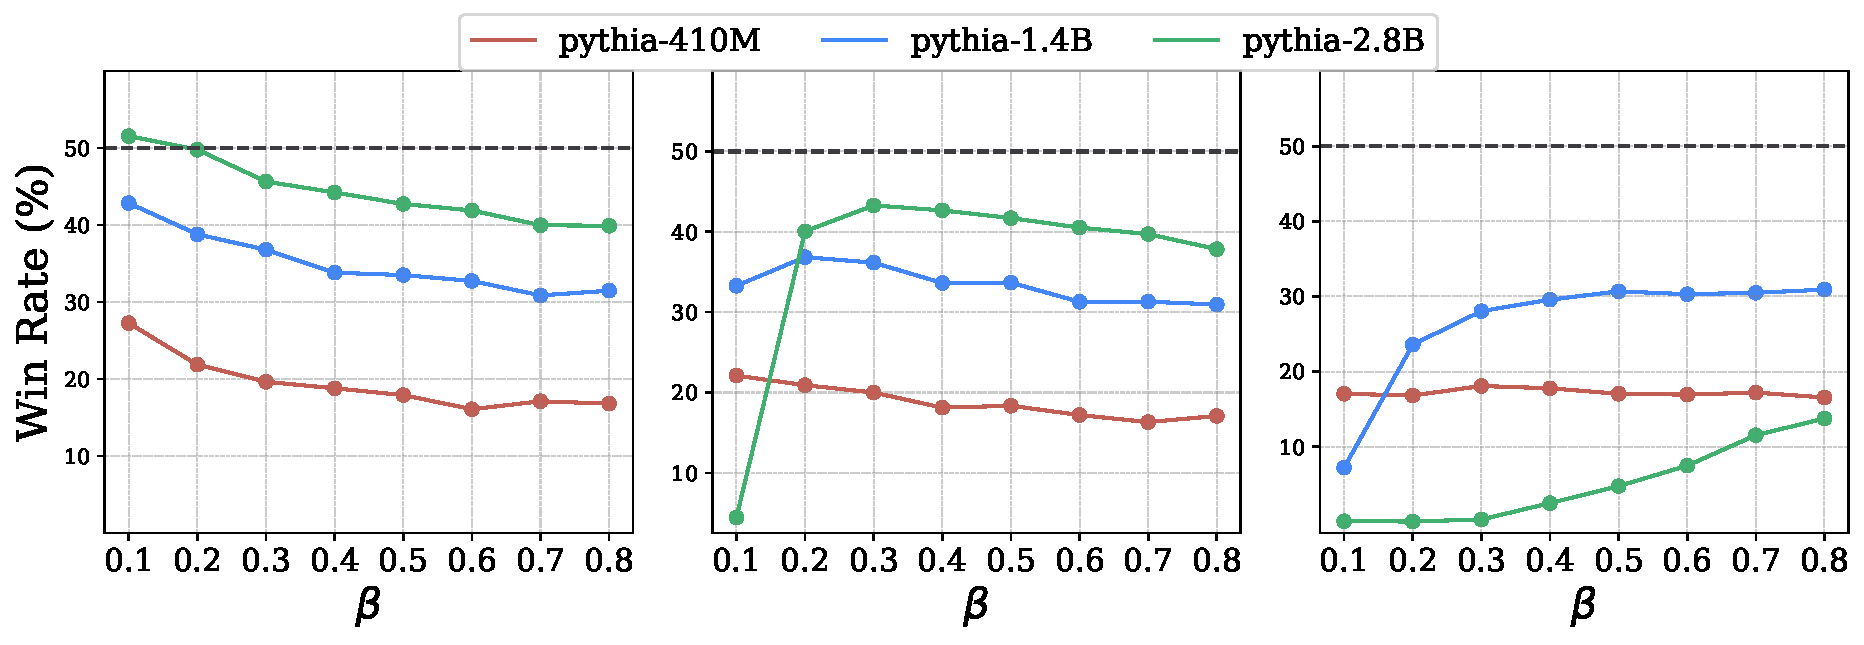
\includegraphics[width=1.0\linewidth]{figs/low_gap_mix_high_gap.pdf}
    % \vspace{-10pt}
    \caption{Win rate performance of DPO across different $\beta$ settings on the \emph{low gap}, \emph{mixed gap}, and \emph{high gap} datasets.}
    \label{fig_low_high_gap}
    \vspace{-10pt}
 \end{figure}
 
\textbf{Models and Metrics.} 
Our study evaluates various model sizes, specifically Pythia-410M, Pythia-1.4B, and Pythia-2.8B \cite{pythia}, to ensure a comprehensive assessment. Following the established protocol in DPO \cite{DPO}, each model iteration undergoes a single epoch with a batch size of 64. This setup provides a uniform basis for evaluation across different models.
We adopt the evaluation strategy from DPO \cite{DPO} to calculate the \textit{win rate}, a metric that measures how often the GPT-4 model prefers a response generated by our models over the default chosen response on the subset of the test dataset.

\textbf{Findings}: 
\textbf{(1) The optimal value of $\beta$ varies with data quality, reflecting divergent performance patterns across datasets.}
In Figure \ref{fig_low_high_gap}, we present the win rate results across three levels of pairwise data gap, each evaluated under varying $\beta$ parameters. As can be observed,
with \emph{low gap} pairwise data, a smaller $\beta$ value is preferable for optimizing performance. This is likely because the informative content of such data allows a lower $\beta$ to facilitate more substantial updates, thereby enhancing alignment accuracy.
Conversely, for \emph{high gap} pairwise data, maintaining a low $\beta$ may lead to overfitting, which significantly undermines the alignment process.
The \emph{mixed gap} dataset --- a combination of both \emph{low gap} and \emph{high gap} datasets --- exhibits a more nuanced performance pattern, suggesting the necessity for a dynamic $\beta$ calibration strategy to adapt to varying data quality.
Consequently, adhering to a fixed $\beta$ value, \ie configuring $\beta$ at the population level, might be inadequate for the dynamic and varied nature of real-world datasets.
\begin{wrapfigure}{r}{0.3\textwidth}
    \centering
    \vspace{-0.45cm}
    \!\!\!\!\!\!\!\! 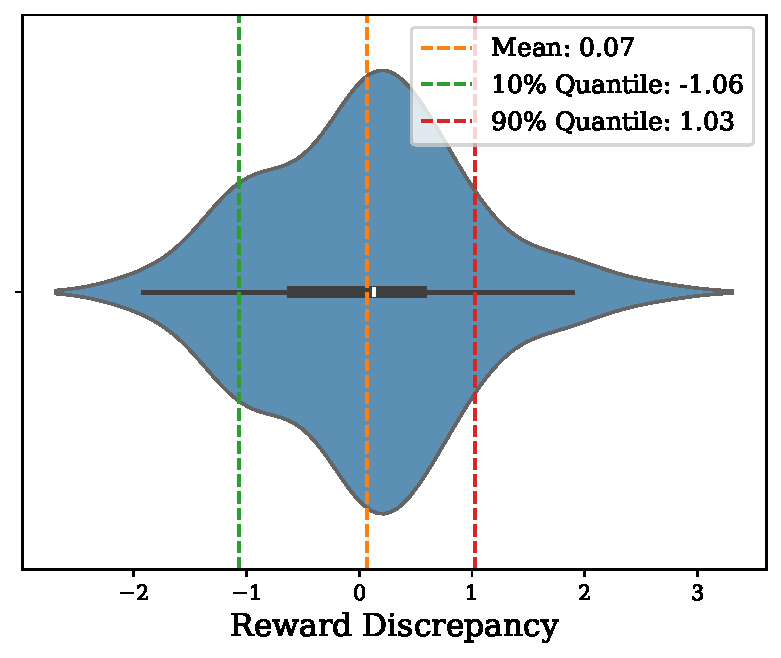
\includegraphics[width=0.32\textwidth]{figs/gap_distribution.pdf}
    \vspace{-0.3cm}
    \caption{The distribution of individual reward discrepancy ($r(\yb_w^{(i)};\xb^{(i)})-r(\yb_l^{(i)};\xb^{(i)})$) on the training dataset of HH.}
    \vspace{-0.5cm}
    \label{fig:gap_distribution}
  \end{wrapfigure}
\textbf{(2) The dataset exhibits notable outliers.} In Figure \ref{fig:gap_distribution}, utilizing the Pythia-2.8B model, we evaluate the data quality by examining the distribution of reward discrepancy for each triplet (which we will define as ``individual reward discrepancy'' later) within the HH dataset's training samples. 
The tails of the density plot extend beyond the highlighted percentiles, suggesting the existence of data samples with significantly higher or lower reward discrepancies.
Notably, cases with significantly higher rewards for positive samples over negative ones suggest low informational value, as these discrepancies likely do not contribute meaningfully to the model's learning process. Whereas the opposite cases hint at potential labeling errors. Both cases deviate from an expected rational distribution range and are thus classified as outliers. For further details on outliers, kindly refer to Appendix \ref{low_gap_high_gap}.

\subsection{Method: Dynamic $\beta$ Calibration in DPO}

Through our empirical analysis, we highlight the sensitivity of DPO to $\beta$ selections and the frequent occurrence of outliers. Hence, 
determining the optimal $\beta$ value requires careful consideration of the quality of pairwise data while also addressing the influence of outliers. This prompts the question: \textit{what criteria define a superior choice of $\beta$?} In response, we propose the following guiding principles:

\textbf{Principle 1:} \textit{The optimal $\beta$ value should be responsive to pairwise data's quality.}

\textbf{Principle 2:} \textit{The selection of $\beta$ value should minimize the influence of outliers.}

\subsubsection{Dynamic $\beta$ Calibration at Batch-Level}
We begin by introducing the concept termed `\textit{individual reward discrepancy}', which represents the difference between the rewards of winning and losing for each triplet, serving as a measurement for pairwise data quality. Formally, for a triplet $(\xb^{(i)}, \yb_w^{(i)}, \yb_l^{(i)}) \in \Set{D}$, the individual reward discrepancy is defined as 
$M_i = r(\yb_w^{(i)};\xb^{(i)}) - r(\yb_l^{(i)};\xb^{(i)}).$
While our primary analysis utilizes the implicit reward model induced by the policy trained using DPO, we also conducted comparative experiments with an explicit reward model. The details of these experiments with the explicit RM can be found in Appendix \ref{sec:appendix_explicit_rm}. For the DPO-based implicit reward model, the reward discrepancy is expressed as:
% To clarify how the reward model is constructed and used, we directly use the implicit reward model induced by the policy trained using DPO. Specifically, the reward discrepancy in DPO is expressed as:

$$ M = \beta_0 \log \left( \frac{\pi_\theta (y_w \mid x) }{\pi_{\text{ref}}(y_w \mid x)} \right) - \beta_0 \log \left( \frac{\pi_\theta (y_l \mid x) }{\pi_{\text{ref}}(y_l \mid x)} \right). $$

Here, \(\pi_\theta\) represents the policy being optimized, and \(\pi_{\text{ref}}\) denotes the reference policy. This formulation captures the difference in the log-probabilities of the winning and losing outcomes, weighted by the parameter \(\beta\).
Motivated by our guiding principles, a straightforward approach is to assign a distinct $\beta$ to each triplet, allowing each $\beta$ to serve as a parameter tailored to its respective triplet. This instance-level dynamic $\beta$ adaption can be formulated as follows:

\begin{eqnarray}
    \begin{aligned}
        \beta_i = \beta_0 + \alpha \large(M_i - M_0 \large) \beta_0 = [1 + \alpha(M_i-M_0)]\beta_0,
    \end{aligned}
    \label{eq:beta}
\end{eqnarray}

where $\beta_0$ represents the benchmark hyperparameter intrinsic to DPO, typically set to 0.1. The term $M_0$ denotes a predetermined threshold, and the coefficient $\alpha$ is a scaling factor within the interval $[0, 1]$ that adjusts the influence of $M_i$ on $\beta_i$. Specifically, when $\alpha = 0$, $\beta_i$ remains constant at $\beta_0$, thus maintaining the standard DPO framework without modification.
% We begin by introducing the concept termed `\textit{individual reward discrepancy}', which represents the difference between the rewards of winning and losing for each triplet, serving as a measurement for pairwise data quality.
% Formally, for a triplet $(\xb^{(i)}, \yb_w^{(i)}, \yb_l^{(i)}) \in \Set{D}$, the individual reward discrepancy is defined as $M_i = r(\yb_w^{(i)};\xb^{(i)})-r(\yb_l^{(i)};\xb^{(i)})$.
% Motivated by our guiding principles, a straightforward approach is to assign a distinct $\beta$ to each triplet, allowing each $\beta$ to serve as a parameter tailored to its respective triplet. This instance-level dynamic $\beta$ adaption can be formulated as follows:
% \begin{eqnarray}
%     \begin{aligned}
%         \beta_i = \beta_0 + \alpha \large(M_i - M_0 \large) \beta_0 = [1 + \alpha(M_i-M_0)]\beta_0,
%     \end{aligned}
%     \label{eq:beta}
% \end{eqnarray}
% where $\beta_0$ represents the benchmark hyperparameter intrinsic to DPO, typically set to 0.1. The term $M_0$ denotes a predetermined threshold, and the coefficient $\alpha$ is a scaling factor within the interval $[0, 1]$ that adjusts the influence of $M_i$ on $\beta_i$. Specifically, when $\alpha = 0$, $\beta_i$ remains constant at $\beta_0$, thus maintaining the standard DPO framework without modification.

Equation \eqref{eq:beta} illustrates that $\beta_i$ increases monotonically with $M_i$, allowing the model to adjust the $\beta$ value based on the running reward differential between paired samples.\
Nevertheless, such instance-level adjustments may introduce instabilities during training. Prior studies have shown that a minibatch approach can help avoid saddle points or local minima \cite{ge2015escaping}, as well as mitigate the impact of noise \cite{robbins1951stochastic, bottou2010large}. Drawing inspiration from these benefits, we propose a batch-level dynamic estimation methodology for $\beta$:

\begin{equation}
    \beta_{\text{batch}} = [1 + \alpha( \EE_{i \sim \text{batch}}[M_i]-M_0)]\beta_0.
\end{equation}
In practical applications, the threshold $M_0$ can be estimated by employing the global mean of $M_i$ with a moving average updating scheme \cite{mae}:
\begin{equation}
    M_0  \leftarrow m M_0 + (1-m)  \EE_{i \sim \text{batch}}[M_i],
    \label{mom}
\end{equation}
where $m\in[0,1)$ is a momentum coefficient.
Such a batch-level calibration method introduces only one new parameter, $\alpha$, to control the scale of $\beta$ adjustment.
The calculation of $\EE_{i \sim \text{batch}}[M_i]$ is straightforward within DPO procedures, thereby incurring no additional computational overhead.


\subsubsection{$\beta$-Guided Data Filtering }
To mitigate the adverse impact of outliers on the $\beta$ selection process, we introduce a $\beta$-guided data filtering mechanism. Informed by $3\sigma$ confidence criterion \cite{3sigma}, this strategy employs a probabilistic model to assess the significance of each triplet $(\xb^{(i)}, \yb_w^{(i)}, \yb_l^{(i)})$ based on its individual reward discrepancy $M_i$, which is defined as:
\begin{equation}
    p(M_i) = \frac{1}{\sqrt{2\pi}\sigma} \exp\left(-\frac{(M_i-M_0)^2}{2\sigma^2}\right),
    \label{sampling_p}
\end{equation}
where $M_0$ and $\sigma$ represent the mean and standard deviation of $M_i$ across the training dataset, respectively.
Similar to the updating scheme of $M_0$ in Equation \eqref{mom}, we dynamically estimate the value of $\sigma$ using the moving average method:
\begin{equation}
     \sigma \leftarrow m \sigma + (1-m)  \sqrt{\mathbb{V}_{i \sim\text{batch}}[M_i]}.
     \label{mom2}
\end{equation}
This probabilistic weighting discerns the relative importance of each sample, guiding the selection of $|\text{batch}| \times \rho$ samples (without replacement) based on their calculated probabilities $p(M_i)$. Here, $\rho$ denotes the selection ratio, defaulting to 0.8, a choice validated by preliminary experiments aimed at optimizing training efficiency and model accuracy.

This process is iterated for each training batch, ensuring that the training data is continuously updated to reflect the most informative samples. The introduction of the $\beta$-guided data filtering strategy is instrumental in fortifying the model against outliers, thereby facilitating the accurate estimation of the $\beta$ value.

\textbf{Highlights:}
We underline the following key features of our proposed $\beta$-DPO framework:
\begin{itemize}[leftmargin=*]
    \item \textbf{Simplicity}: $\beta$-DPO is extremely straightforward and quick to implement. It merely involves a dynamic $\beta$ adjustment at the batch level and a $\beta$-guided data filtering mechanism, both of which are predicated upon the reward discrepancy denoted by $M_i$.
    \item \textbf{Efficiency}: Unlike other methodologies \cite{RSO,morimura2024filtered,pruthi2020estimating,f-dpo} that necessitate an additional gold model for data filtering, our method leverages the running reward discrepancy $M_i$ within the DPO framework. Moreover, our empirical studies indicate that $\beta$-DPO exhibits insensitivity to the hyperparameters $\rho$. A default setting of $\rho=0.8$ typically yields satisfactory performance.
    \item \textbf{Model-agnostic}: As a variant of the traditional DPO, the proposed $\beta$-DPO can function as a plug-and-play module. It allows straightforward integration of future enhancements and extensions within the DPO framework. Our empirical investigations corroborate this assertion.
\end{itemize}

\subsection{Discussion with Previous Studies}
\textbf{Relations to Data Selection.} An increasing volume of works \cite{RSO,morimura2024filtered,LIMA,pruthi2020estimating, xia2024less} have underscored the impact of data quality on the performance of LLM's alignment. A common practice among these efforts involves employing a so-called ``gold model'' for data selection. This approach, however, introduces significant computational demands and the choice of the gold model directly influences the resultant system's performance. The focus of this work, it should be noted, is not to propose a superior strategy for data selection. Instead, we aim to enhance adaptability to the quality of data by dynamically adjusting the $\beta$ parameter. This adjustment facilitates improved $\beta$ estimation by selecting data based on the reward. Moreover, Section \ref{exp_adaptation} illustrates the compatibility of dynamic $\beta$ adjustment with other data selection methodologies.

\textbf{Relations to Recent Temperature Schemes.}
Dynamic temperature frameworks have been introduced in the realm of contrastive learning, motivated by various objectives, such as addressing out-of-distribution tasks \cite{Uncertainty} or accommodating long-tail data distributions \cite{long_tail}. The work most closely related to ours, MACL \cite{MACL}, has indeed proposed an alignment-adaptive strategy; however, its primary aim was to navigate the uniformity-tolerance dilemma. Hence, the integration of dynamic temperature mechanisms with LLM's alignment remains an underexplored area against this backdrop.
\section{Experiments}
\label{Experiments}
\begin{figure}[t]
    \centering
    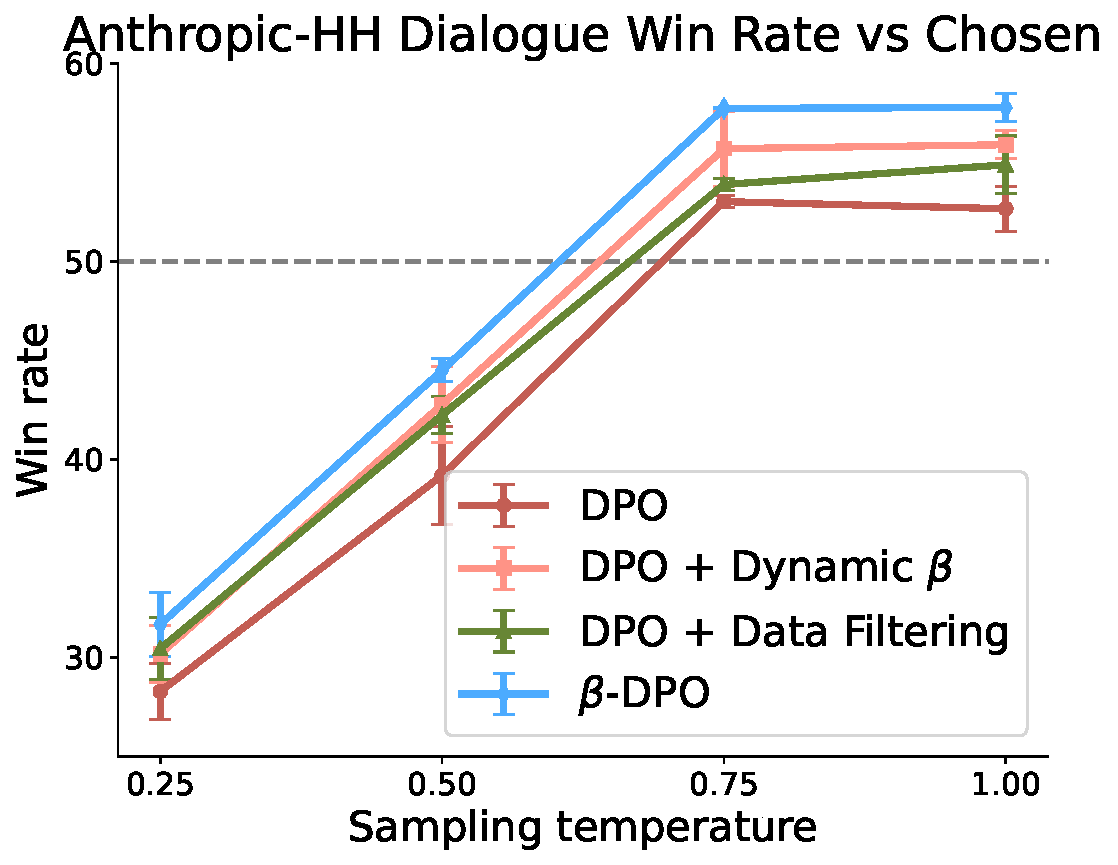
\includegraphics[width=0.49\textwidth]{figs/win_rate_hh.pdf}
    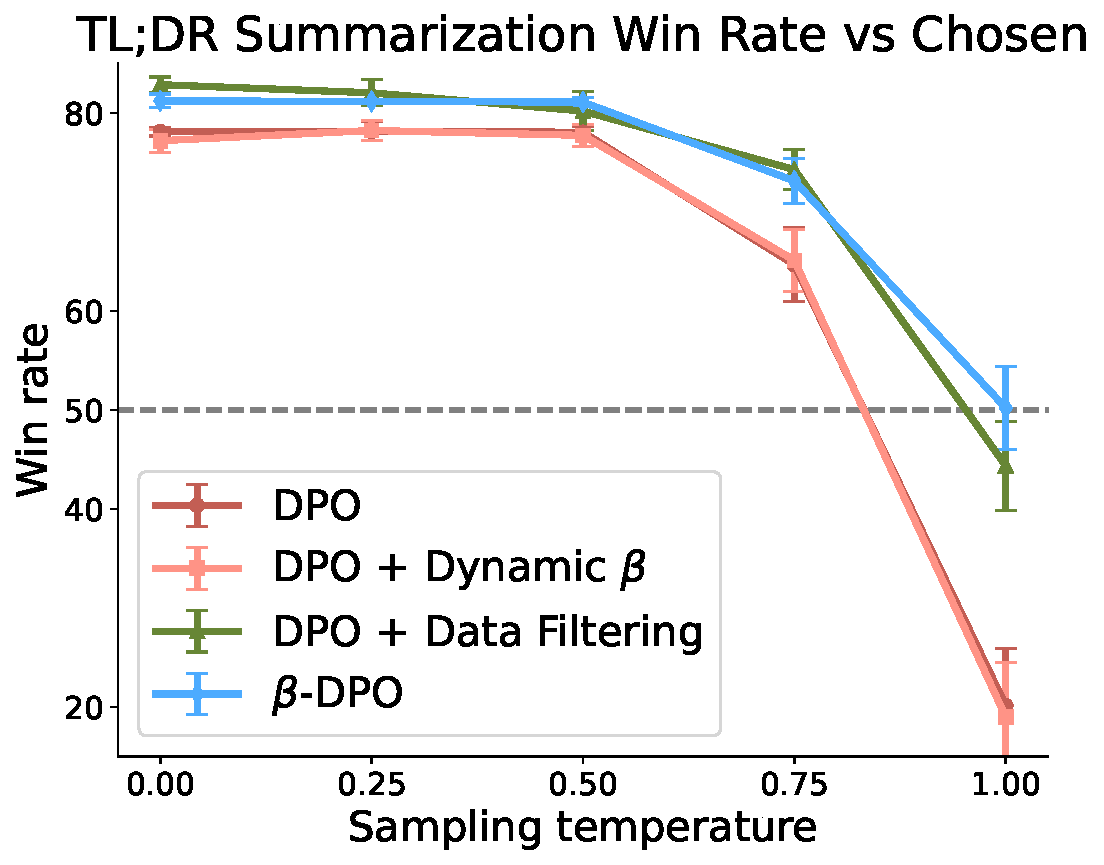
\includegraphics[width=0.49\textwidth]{figs/win_rate_tldr.pdf}
    \caption{
    \textbf{Left.} 
    The win rates computed by GPT-4 evaluations for the Anthropic-HH one-step dialogue; $\beta$-DPO consistently outperforms across all sampling temperatures.
    \textbf{Right.} 
    In the comparison of TL;DR summarization win rates versus chosen summaries with GPT-4 as the evaluator, $\beta$-DPO is distinguished as the only strategy achieving a win rate over 50\% across different sampling temperatures.
    }
    \label{fig:dialogue-main}
\end{figure}

In this section, we commence by conducting an empirical evaluation of $\beta$-DPO on two specific tasks: dialogue generation and summarization. Subsequently, we analyze the various adaptations of the proposed method $\beta$-DPO. Concluding this section, we underscore the imperative need for batch-level dynamic $\beta$ calibration, highlighting its significance in the context of our study.

\subsection{Empirical Evaluation of $\beta$-DPO on Dialogue Generation and Summarization}
\textbf{Datasets and Setup.} Our experiments are conducted on the Anthropic HH dataset \cite{Bai2022training} and Reddit TL;DR summarization dataset \cite{tldr_dataset}. The training configuration follows from \citet{DPO}. The goals of these experiments are to study: 1) How $\beta$-DPO performs on single-turn dialogue generation and summarization tasks; 2) How the sampling temperature affects the performance of $\beta$-DPO; 3) How $\beta$-DPO works with different model sizes. For detailed experimental settings, please refer to Appendix \ref{setup_exp}.

\textbf{Baselines.} In our comparison, we examine the performance of $\beta$-DPO relative to its counterparts: the standard DPO, DPO implemented with a dynamic $\beta$ yet devoid of $\beta$-guided data filtering, and DPO complemented by data filtering with $\beta$ fixed at 0.1.
% We compare $\beta$-DPO with DPO, DPO with dynamic $\beta$ (without $\beta$-guided data filtering), DPO with data filtering (keep $\beta$ as 0.1).

\textbf{Win Rate Across different Sampling Temperature.} An analysis of win rates derived from GPT-4 evaluations on the Anthropic-HH one-step dialogue demonstrates that $\beta$-DPO consistently outperforms across all sampling temperatures, as depicted in Figure \ref{fig:dialogue-main} (Left). Furthermore, for the TL;DR summarization task, $\beta$-DPO stands out as the only approach achieving win rates above 50\% for diverse sampling temperatures, which is visually represented in Figure \ref{fig:dialogue-main} (Right). The data also suggests that while both dynamic $\beta$ and data filtering enhance DPO's effectiveness, the impact of data filtering is especially pronounced in the summarization task, likely due to the inherently greater noise present in the Reddit TL;DR summarization dataset. Notably, $\beta$-DPO exhibits a remarkable degree of robustness to variations in sampling temperature. As the temperature incrementally escalates from 0.0 to 1.0, the win rate for standard DPO plunges to a mere 25\%, whereas $\beta$-DPO maintains a commendable performance level with a win rate of 54\%.

% \textbf{Win rate across different sampling temperature:} The win rates generated through GPT-4 evaluations for the Anthropic-HH one-step dialogue reveal that $\beta$-DPO consistently leads across all sampling temperature, as shown in Figure \ref{fig:dialogue-main} (left). On the TL;DR summarization task, $\beta$-DPO emerges as the sole methodology attaining a win rate exceeding 50\% across various sampling temperatures, as illustrated in Figure \ref{fig:dialogue-main} (right). In addition, we observe that dynamic $\beta$ and data filtering both can improve the performance of DPO, but data filtering is more significant in the summarization task. We attribute this to the fact that the Reddit TL;DR summarization dataset is more noisy than the Anthropic HH dataset. Moreover, we find $\beta$-DPO to be much more robust to the sampling temperatures, while sampling temperature increase from 0.0 to 1.0, DPO's win rate decreases to 25\%, while $\beta$ DPO still achieve 54\%.

\textbf{Win Rate Across Different Model Sizes.} We further evaluate the performance of $\beta$-DPO on the Anthropic HH dataset with Pythia-410M, -1.4B, and -2.8B models. The results are summarized in Table \ref{tab:ablation}. We observe that $\beta$-DPO consistently outperforms DPO, DPO with dynamic $\beta$, and DPO with data filtering across all model sizes.
We observe that in a smaller model, the improvement of data filtering is more significant, while in a larger model, the improvement of dynamic $\beta$ is more significant. We attribute this to the fact that the larger model has more capacity to learn the optimal policy, while the smaller model needs more help from the data filtering.



\begin{table}
    \centering
    \caption{
    % Win rate comparison on the Anthropic HH dataset with Pythia-410M, -1.4B, and -2.8B models. using GPT-4 as evaluator.
    Win rate comparison of Pythia-410M, -1.4B, and -2.8B models on the Anthropic HH dataset, evaluated using GPT-4.
    }
    \begin{tabular}{l|l|l|l}
        \toprule
        \textbf{Method} & \textbf{410M} & \textbf{1.4B} & \textbf{2.8B} \\
        \midrule
        DPO & $26.19$ & $42.78$ & $51.51$ \\
        DPO + Dynamic $\beta$ & $27.15^{\color{+}+ 3.67\%}$ & $43.51^{\color{+}+ 1.71\%}$ & $55.19^{\color{+}+ 7.14\%}$ \\
        DPO + Data Filtering & $29.03^{\color{+}+ 10.84\%}$ & $46.99^{\color{+}+ 9.84\%}$ & $53.42^{\color{+}+ 3.71\%}$ \\
        $\beta$-DPO & $30.18^{\color{+}+ 15.23\%}$ & $48.67^{\color{+}+ 13.77\%}$ & $57.07^{\color{+}+ 10.79\%}$ \\
        \bottomrule
    \end{tabular}
    \label{tab:ablation}
\end{table}




% We further investigate the performance of $\beta$-(IPO, KTO, SPPO) 
% In our work, we introduce a dynamic $\beta$ strategy, termed $\beta$-DPO, aimed at refining the decision process in the classical DPO framework and its variants: IPO, KTO, and SPPO. Our evaluation on the Anthropic HH dataset illustrates that, among the original variants, IPO outshines KTO and SPPO in terms of performance. By implementing our dynamic $\beta$ technique, creating dynamic versions: $\beta$-IPO, $\beta$-KTO, and $\beta$-SPPO, every variant witnesses a notable improvement in efficacy. Specifically, $\beta$-IPO demonstrates a significant performance leap of 17.9\%. This evidence solidly supports that the dynamic $\beta$ approach not only integrates seamlessly with existing DPO variants but also markedly propels their performance forward, offering a robust method for the advancement of language models trained with human feedback.

% \textbf{$\beta$-DPO adapts to and improves upon existing DPO's variants} 
% We further investigate the performance of $\beta$-(IPO, KTO, SPPO) across various DPO variants. As seen in Figure \ref{fig:gradient} (right),  it becomes apparent that neither KTO nor SPPO exhibits superiority over IPO when trained on the Anthropic HH dataset. Furthermore, our integration of the $\beta$ parameter into these models—IPO, KTO, SPPO—manages to enhance the performance of these DPO variants considerably. Notably, $\beta$-IPO registers a profound improvement of 17.9\%. These results strongly indicate that the $\beta$-augmented models—IPO, KTO, SPPO—constitute an adaptive and efficacious strategy for the development of language models trained via human feedback.
% KTO and SPPO is not superior to IPO on the Anthropic HH dataset. Besides, our $\beta$-(IPO, KTO, SPPO) still could improve the performance of these DPO variants, where $\beta$-IPO achieves significant 17.9\% improvement. This suggests that $\beta$-(IPO, KTO, SPPO) is a adaptive and effective method for training language models with human feedback. 
% \begin{table}
%     \centering
%     \caption{Ablation study of $\beta$-DPO on the Anthropic HH dataset using GPT-4 as evaluator.}
%     \begin{tabular}{l|l}
%         \toprule
%         \textbf{Method} & \textbf{Win Rate} \\
%         \midrule
%         IPO & $52.05$ \\
%         $\beta$-IPO & $54.73^{\color{+}+ 5.15\%}$ \\
%         \midrule
%         ORPO & $36.11$ \\
%         $\beta$-ORPO & $38.60^{\color{+}+ 6.90\%}$ \\
%         \bottomrule
%     \end{tabular}
%     \label{tab:ipo_orpo}
% \end{table}





\subsection{Adaptations of $\beta$-DPO}
\label{exp_adaptation}
In this section, our inquiry is twofold: first, we aim to understand the performance of $\beta$-DPO when applied across various filtering strategies; second, we examine its efficacy across different adaptations of the DPO framework. In terms of filtering strategies, prevailing studies \cite{pruthi2020estimating, xia2024less} in the domain largely employ a gradient-based approach. We propose to extend this methodology into three distinct scenarios. This involves arranging the gradients of pairwise data within a batch and consequently: (1) Excluding the top 20\% of samples, hereby referred to as \textbf{Filter Head},
(2) Excluding the bottom 20\% of samples, hereby referred to as \textbf{Filter Tail},
(3) Excluding both the top and bottom 10\% of samples, a method we denote as \textbf{Filter Tail \& Head}.
For a fair comparison, we maintain the amount of data excluded at 20\% for the above strategies.
Second, we integrate three variants of DPO into our analysis: the IPO \cite{ipo}, a novel approach that facilitates learning directly from preferences without the need for the Bradley-Terry (BT) model. Additionally, we consider the KTO \cite{KTO}, which focuses on discerning whether a preference is desirable or undesirable and SPPO \cite{sppo}, which approximates the Nash equilibrium. For detailed settings, we refer the reader to the supplementary material.

\textbf{Selective filtering of the top 20\% of samples markedly enhances model performance. } This approach, detailed in Figure \ref{fig:gradient} (Left), not only surpasses other filtering strategies but also suggests that these samples, which exhibit the smallest discrepancies between positive and negative pairs, are particularly prone to flipped noise. By excluding them, the model's learning efficacy is appreciably improved.

\textbf{Dynamic $\beta$ adapts to and improves upon existing filtering strategies.} Figure \ref{fig:gradient} (Left) corroborates our stance that a static $\beta$ proves insufficient within the DPO framework. We contend that the application of our dynamic $\beta$-DPO could markedly reshape the DPO field by fostering the development of advanced filtering techniques.

\textbf{Dynamic $\beta$ Enhancement across DPO Variants.}
We introduce dynamic $\beta$-DPO, a novel strategy enhancing DPO and its variants: IPO, KTO, and SPPO in Figure \ref{fig:gradient} (Middle). Our results on the Anthropic HH dataset demonstrate that while IPO initially leads in performance, the integration of dynamic $\beta$ substantially elevates all variants, notably increasing $\beta$-IPO's efficiency by 17.9\%. This underscores dynamic $\beta$-DPO's capability to significantly enhance model training through adaptable improvements, solidifying its value in advancing language models via human feedback.
% \begin{figure}
%     \centering
%     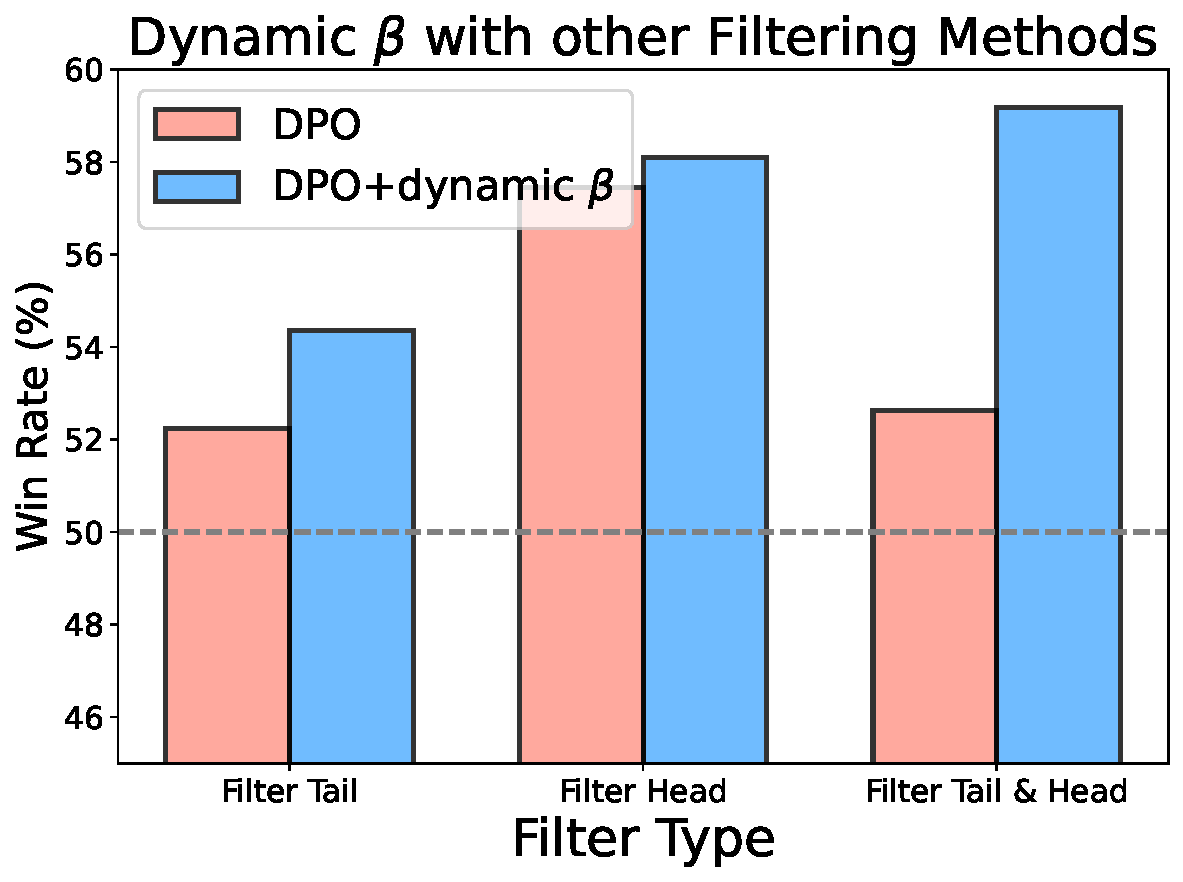
\includegraphics[width=0.4\textwidth]{figs/filter_gradient.pdf}
%     \includegraphics[width=0.4\textwidth]{figs/KTO-SPPO.pdf}
%     \caption{
%     \textbf{Left.} The win rates generated through GPT-4 evaluations for the Anthropic-HH single-turn dialogue reveal that $\beta$-DPO could adapt to various filtering strategies.
%     \textbf{Right.} The $\beta$-DPO approach win rates across different DPO variants, using GPT-4 as evaluator.}
%     % TL;DR summarization win rates vs. chosen summaries, using GPT-4 as evaluator; $\beta$-DPO emerges as the sole methodology attaining a win rate exceeding 50\% across various sampling temperatures.}
%     % \vspace{-2mm}
%     \label{fig:gradient}
% \end{figure}

\begin{figure}
    \centering
    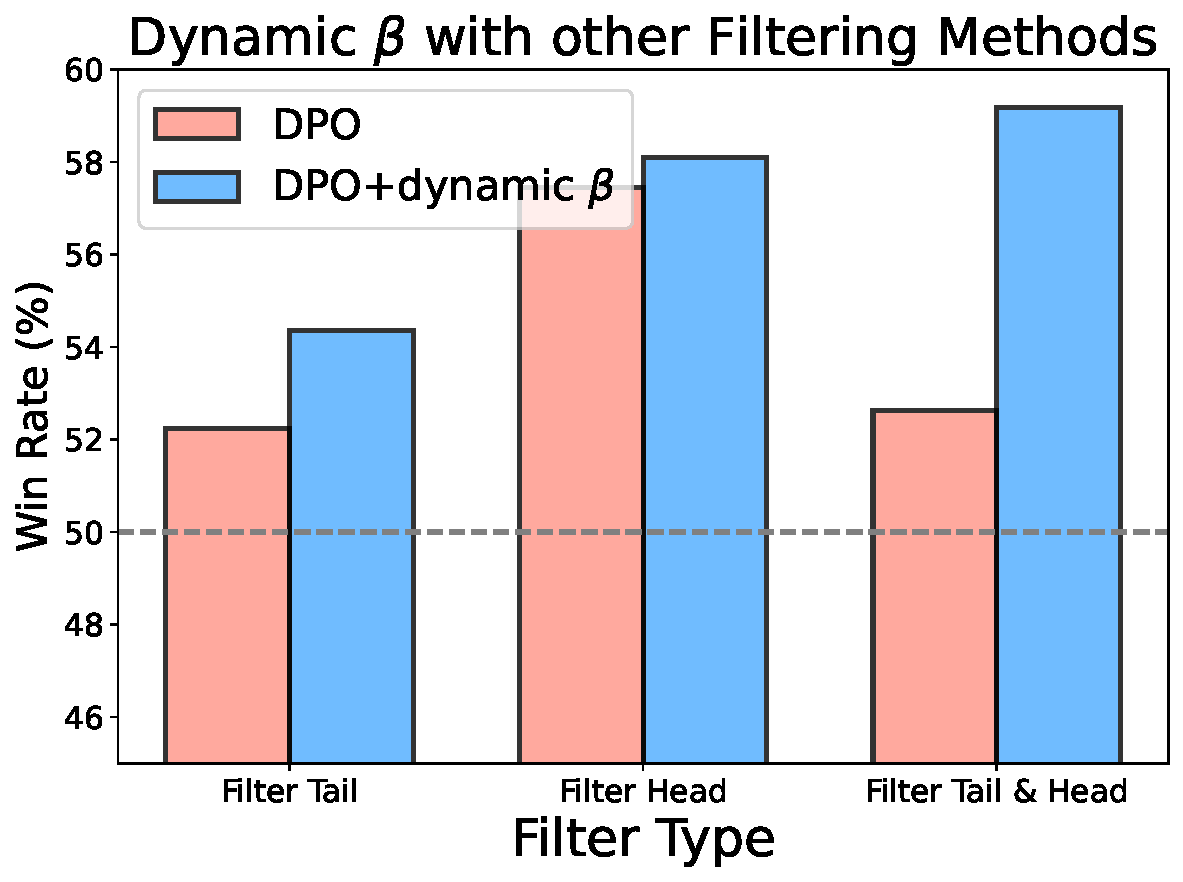
\includegraphics[width=0.32\textwidth]{figs/filter_gradient.pdf}
    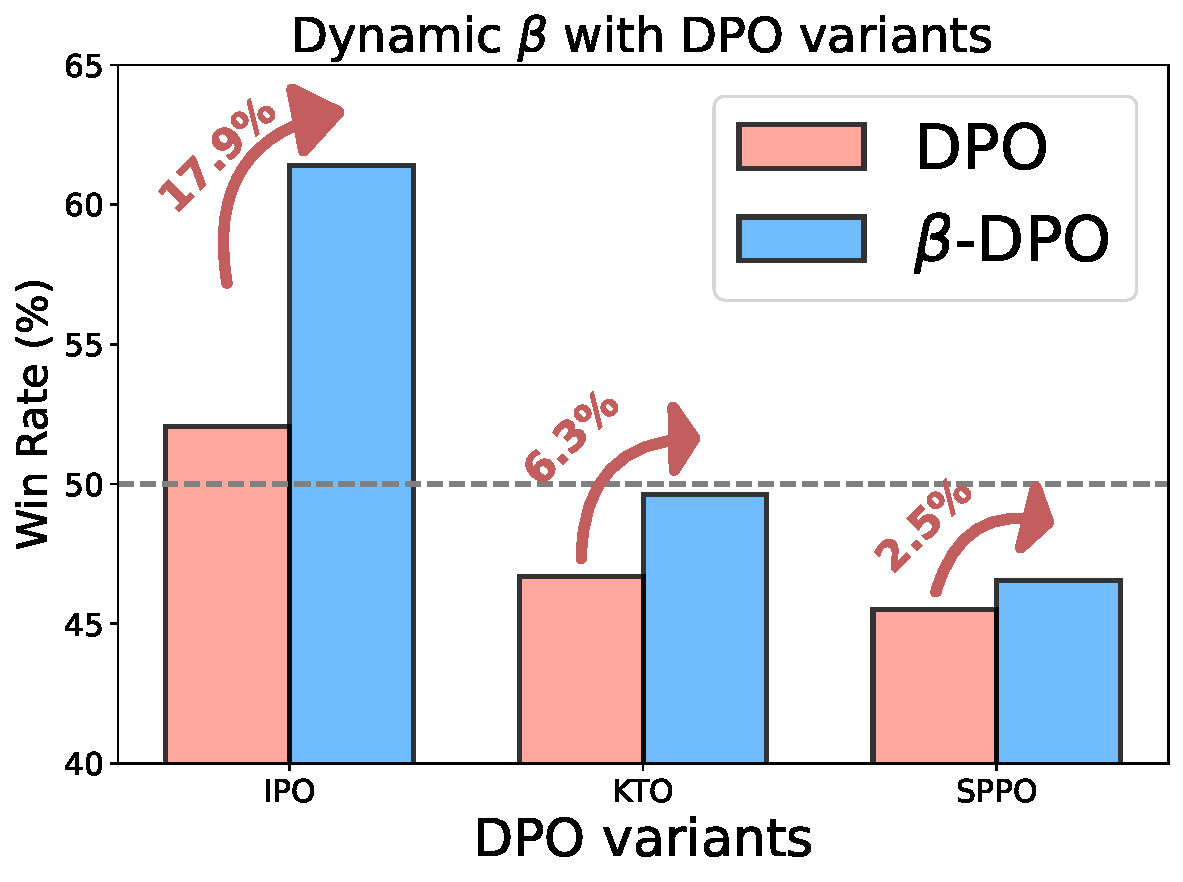
\includegraphics[width=0.32\textwidth]{figs/kto-sppo.pdf}
    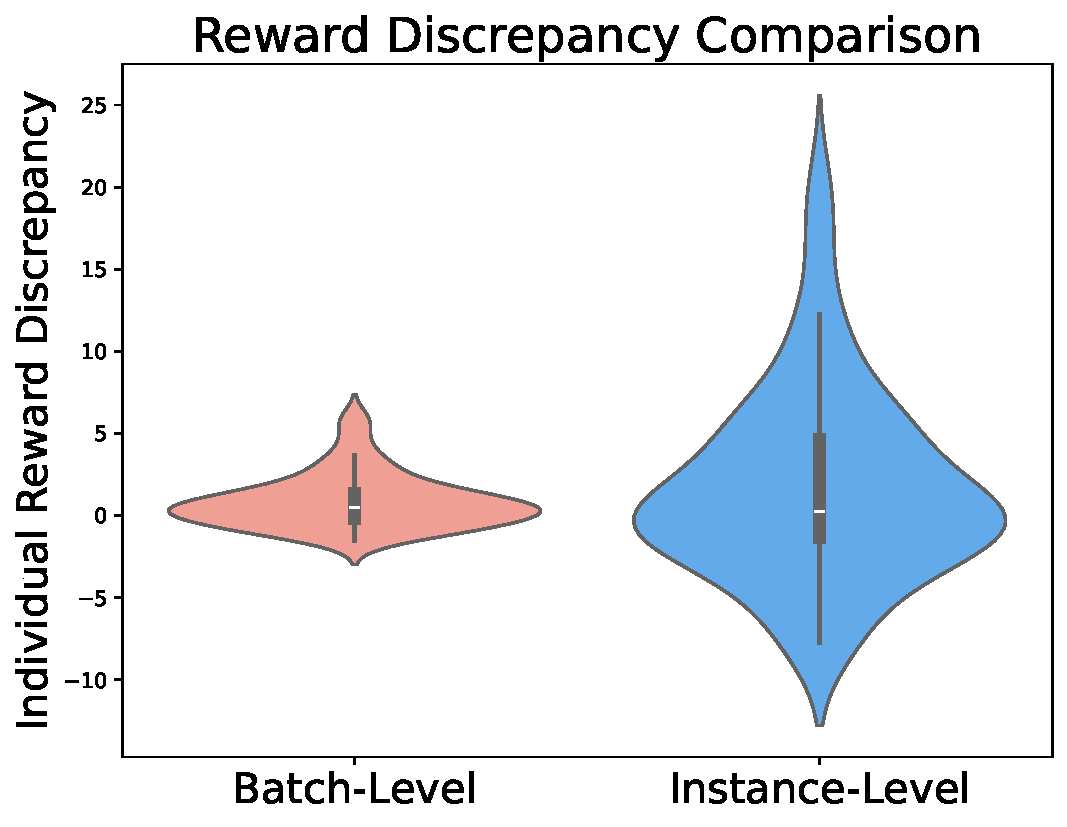
\includegraphics[width=0.32\textwidth]{figs/gap_batch_instance.pdf}
    \caption{
    \textbf{Left:} Win rates from GPT-4 evaluations on Anthropic-HH single-turn dialogues, showcasing $\beta$-DPO's adaptability to diverse filtering strategies. \textbf{Middle:} Win rates of $\beta$-DPO across various DPO variants as evaluated by GPT-4. \textbf{Right:} Distribution of individual reward discrepancies following fine-tuning through batch-level and instance-level calibration.
    % \textbf{Left:} The win rates generated through GPT-4 evaluations for the Anthropic-HH single-turn dialogue reveal that $\beta$-DPO could adapt to various filtering strategies.
    % \textbf{Middle:} The $\beta$-DPO approach win rates across different DPO variants, using GPT-4 as evaluator.
    % \textbf{Right:} The distribution of individual reward discrency after fined-tuned by batch-level calibration and instance-level calibration.
    }
    
    % TL;DR summarization win rates vs. chosen summaries, using GPT-4 as evaluator; $\beta$-DPO emerges as the sole methodology attaining a win rate exceeding 50\% across various sampling temperatures.}
    % \vspace{-2mm}
    \label{fig:gradient}
\end{figure}


\subsection{Necessity of Batch-Level Dynamic $\beta$ Calibration}
\label{sec_batch_level}
In this section, we aim to underscore the pivotal role of batch-level tuning in calibrating the parameter $\beta$. To this end, we compare the performance of our $\beta$-DPO algorithm under two distinct regimes: one employing batch-level dynamic $\beta$ calibration, and the other utilizing instance-level dynamics. To emulate the diverse data disparity scenarios encountered in practical applications, we adopt the methodology outlined in Section \ref{motivation_sec}, meticulously blending datasets characterized by both \emph{low gap} and \emph{high gap} attributes at varying ratios.

\textbf{Batch-level calibration surpasses both instance-level and population-level approaches.} The results presented in Table \ref{tab:noise} illustrate that batch-level dynamic $\beta$ calibration yields superior performance compared to instance-level dynamics and the baseline population-level approach (referred to as vanilla DPO) across a range of mixture ratios. This improvement can be credited to the batch-level calibration's ability to adjust to the varying data quality present within a batch, thus refining the model's learning process.
Conversely, instance-level dynamics can provoke excessively vigorous model updates, precipitating a decline in performance particularly noticeable at a mixture ratio of 40\%, a scenario in which outliers exert a significant negative impact.

\textbf{Instance-level calibration magnifies the impact of outliers.}
As demonstrated in Figure \ref{fig:gradient} (Right), instance-level calibration can inadvertently widen the range of reward discrepancy distribution. This broadened range suggests that instance-level calibration might be leading to excessively high or low $\beta$ values for the model. Such disparities in $\beta$ values consequently cause disproportionate update rates for certain samples, further intensifying the extremities in the distribution. 
\begin{table}
    \centering
    \caption{
    Comparison of win rates across varying mixture ratios on the Anthropic HH dataset, with each ratio indicating the proportion of \emph{high-gap} to \emph{low-gap} datasets, e.g., a 40\% mixture ratio reflects a blend of 40\% \emph{high-gap} and 60\% \emph{low-gap}.
    }
    \begin{tabular}{l|l|l|l|l}
        \toprule
        \textbf{Mixture Ratio} & \textbf{10\%} & \textbf{20\%} & \textbf{30\%} & \textbf{40\%}\\
        \midrule
        Vanilla DPO & $50.17$ & $50.56$ & $47.95$ & $29.15$ \\
        + Instance-level calibration & $49.18^{\color{-}- 1.97\%}$ & $49.82^{\color{-}- 1.46\%}$ & $44.42^{\color{-}- 7.36\%}$ & $16.82^{\color{-}- 42.30\%}$ \\
        + Batch-level calibration & $57.68^{\color{+}+ 14.69\%}$ & $56.15^{\color{+}+ 11.06\%}$ & $51.25^{\color{+}+ 6.88\%}$ & $34.92^{\color{+}+ 19.79\%}$ \\
        \bottomrule
    \end{tabular}
    \label{tab:noise}
\end{table}

% \setlength{\tabcolsep}{6pt}

\textbf{Our $\beta$-calibration strategy consistently outperforms baseline methods.} To expand our approach to more diverse datasets and model sizes, we follow the current state-of-the-art models SimPO \cite{SimPO2024}. We perform $\beta$-DPO with two families of models, Llama3-8B \citep{llama3modelcard}, Mistral2-7B \citep{Jiang2023Mistral7}, on the \href{https://huggingface.co/datasets/HuggingFaceH4/ultrachat_200k}{UltraChat-200k} dataset~\cite{Ding2023EnhancingCL}. For comparison with baselines, we assess our models using one of the most popular open-ended instruction-following benchmarks: AlpacaEval 2. All settings are consistent with SimPO \cite{SimPO2024}.
\begin{wraptable}[11]{r}{7.7cm}
\centering
\vspace{-0.6em}
\caption{Performance comparison of different models}
 \small
\resizebox{7.7cm}{!}{
\begin{tabular}{ccccc}
\toprule
\multirow{2}{*}{Model} & \multicolumn{2}{c}{Mistral-Instruct (7B)} & \multicolumn{2}{c}{Llama3-Instruct (8B)} \\
\cmidrule(lr){2-3} \cmidrule(lr){4-5}
 & LC (\%) & WR (\%) & LC (\%) & WR (\%) \\
\midrule
DPO & 20.98 & \textbf{21.60} & 40.44 & 37.38 \\
$\beta$-DPO & \textbf{23.56} & 20.42 & \textbf{43.38} & \textbf{38.21} \\
\midrule
SimPO & 28.50 & 30.56 & 44.38 & 38.97 \\
$\beta$-SimPO & \textbf{30.48} & \textbf{32.13} & \textbf{46.03} & \textbf{40.18} \\
\bottomrule
\end{tabular}
}
\label{tab:performance_comparison_lc}
\end{wraptable}
Table \ref{tab:performance_comparison_lc} presents the AlpacaEval 2 results under the Mistral-Instruct (7B) and Llama3-Instruct (8B) settings. LC and WR denote length-controlled and raw win rate, respectively. Regardless of whether we use Llama3-8B or Mistral-7B, and whether the loss function is DPO or SimPO, our $\beta$-{D, Sim}PO strategy consistently demonstrates significant performance improvements. This thoroughly showcases the method's strong generalization ability and excellent scalability.
% \begin{table}[h!]
% \centering
% \begin{tabular}{ccccccccccc}
% \hline
% % Method & DPO & $\beta$-DPO  & SimPO  & $\beta$-SimPO & SimPO & $\beta$-SimPO & $\beta$-SimPO & SimPO & $\beta$-SimPO & $\beta$-SimPO  \\
% % RM &implicit & implicit &implicit & implicit & PairRM & PairRM & PairRM & ArmoRM &ArmoRM &ArmoRM \\
% &BL & BL &BL & BL & BL & IL & BL & BL & IL & BL\\
% \hline
% LC (\%) & 40.44 & \textbf{43.38} & 44.38 & \textbf{46.03} & 44.7 & 43.84 & \textbf{45.65} & 53.7 & 49.05 & \textbf{54.86} \\
% \hline
% WR (\%) & 37.38 & \textbf{38.21} & 38.97 & \textbf{40.18} & 38.98 & 38.54 & \textbf{39.76} & 47.50 & 45.47 & \textbf{49.66} \\
% \hline
% \end{tabular}
% \caption{Performance comparison of different methods}
% \label{tab:performance_comparison}
% \end{table}


\section{Conclusion and Future Work}
\label{conclusion}
This paper introduces $\beta$-DPO, a novel framework designed to optimize DPO by dynamically adjusting the $\beta$ parameter in response to the variability in the informativeness of pairwise data. Our approach, which incorporates $\beta$-guided data filtering and batch-level dynamic $\beta$ calibration, has demonstrated significant improvements in DPO's performance across a range of models and datasets. The empirical evaluations indicate that $\beta$-DPO offers an adaptable training paradigm for LLMs with human feedback.

\textbf{Limitations and Future Work.}
Our work on $\beta$-DPO showcases a promising framework for LLM optimization, albeit with room for advancement. Future endeavors should explore:
Adaptive $\beta$ in Self-Play: Extending $\beta$-DPO to self-play scenarios \cite{spin,sppo} where negative samples dynamically adapt, necessitating iterative $\beta$ adjustments, to foster the evolution of superior model strategies.
Enhanced Evaluation Standards: Development of sophisticated metrics and use of advanced evaluators beyond win rates, capitalizing on advancements like GPT-4+, to comprehensively gauge model performance.
Scalability Investigation: Examining $\beta$-DPO's scalability to ultra-large models surpassing 7B parameters, and its integration into diverse DPO-inspired architectures, is pivotal for practical impact.
Automated Parameter Tuning: Pursuing automation in parameter tuning, alleviating manual intervention for $\beta$, to streamline the training pipeline and broaden accessibility.

\begin{ack}
This research is supported by the National Science and Technology Major Project (2023ZD0121102), National Natural Science Foundation of China (92270114, 62302321). This research was also supported by the advanced computing resources provided by the Supercomputing Center of the USTC.
\end{ack}

\bibliography{neurips_2024}
\bibliographystyle{abbrvnat}
% \section*{References}


% References follow the acknowledgments in the camera-ready paper. Use unnumbered first-level heading for
% the references. Any choice of citation style is acceptable as long as you are
% consistent. It is permissible to reduce the font size to \verb+small+ (9 point)
% when listing the references.
% Note that the Reference section does not count towards the page limit.
% \medskip


% {
% \small


% [1] Alexander, J.A.\ \& Mozer, M.C.\ (1995) Template-based algorithms for
% connectionist rule extraction. In G.\ Tesauro, D.S.\ Touretzky and T.K.\ Leen
% (eds.), {\it Advances in Neural Information Processing Systems 7},
% pp.\ 609--616. Cambridge, MA: MIT Press.


% [2] Bower, J.M.\ \& Beeman, D.\ (1995) {\it The Book of GENESIS: Exploring
%   Realistic Neural Models with the GEneral NEural SImulation System.}  New York:
% TELOS/Springer--Verlag.


% [3] Hasselmo, M.E., Schnell, E.\ \& Barkai, E.\ (1995) Dynamics of learning and
% recall at excitatory recurrent synapses and cholinergic modulation in rat
% hippocampal region CA3. {\it Journal of Neuroscience} {\bf 15}(7):5249-5262.
% }


%%%%%%%%%%%%%%%%%%%%%%%%%%%%%%%%%%%%%%%%%%%%%%%%%%%%%%%%%%%%
\newpage
\appendix
% \section{Appendix}
\section{Experiment}
\label{exp_appendix}
\subsection{$\beta$-DPO Implementation Details and Hyperparameters}
\label{setup_exp}
$\beta$-DPO is relatively straightfoward to implement; The full algorithm is summarized in Algorithm \ref{alg}.
% The  for the $\beta$-DPO loss is provided below:

\begin{algorithm}[h]
    \caption{$\beta$-Direct Preference Optimization}\label{alg:beta-dpo}
    \begin{algorithmic}[1]
    \REQUIRE Preference dataset $\mathcal{D}$, batch size $b$, constraint coefficient $\beta_0$, selection ratio $\rho$, scaling factor $\alpha$, and learning rate $\eta$.
    \STATE Initialize model $\pi_{\theta_0}$ with supervised finetuning on $\mathcal{D}$.
    % \FOR{$n=1\ldots N$ iterations}
    \WHILE{not converged}
        \STATE Sample a batch $\mathcal{B} = \{(\xb^{(i)}, \yb_w^{(i)}, \yb_l^{(i)})\}_{i=1}^b$ from $\mathcal{D}$.
        \STATE Compute the individual reward discrepancy $M_i = r(\yb_w^{(i)};\xb^{(i)})-r(\yb_l^{(i)};\xb^{(i)})$.
        \STATE Update the threshold $M_0$ and $\sigma$ using Equations \eqref{mom} and \eqref{mom2}.
        \STATE Sample $b \times \rho$ samples without replacement based on $p(M_i)$ in Equation \eqref{sampling_p}.
        \STATE Compute the batch-level $\beta$ using Equation~\eqref{eq:beta}.
        \STATE Compute the loss using the Equation~\eqref{eq:DPO2}.
        \STATE Compute the gradient and update the model $\theta_t \leftarrow \theta_{t-1} - \eta \nabla_\theta  \ell(\theta_{t-1}, \mathcal{B})$.
    \ENDWHILE
    % \ENDFOR
\RETURN Final model $\pi_{\theta}$.
\end{algorithmic}
\label{alg}
\end{algorithm}

Unless noted otherwise, we use a $\beta=0.1$, batch size of 64, $m=0.9$ to ensure the stability of the global $M_i$ estimation, $\rho=0.8$ to filter 20\% uninformative samples, and the Adam optimizer with a learning rate $5e-7$ by default.  We carried out all computational tasks on a suite of four 80GB A100 GPUs. For the Pythia-410M model, we use a batch size of 128, while the rest of the parameters remain the same.

% In paticular, for \textbf{single-turn dialugue} , we utilize \textbf{Pythia-2.8, -1.4b and -410M} to conduct the experiments on Anthropic-HH dataset. In this setting, no pre-trained SFT model is available; we therefore fine-tune an off-the-shelf language model on the only the preferred completions to form the SFT model. As for \textbf{summarization}, we use the Reddit TL;DR summarization dataset along with human preferences gatherd by \citet{tldr2}. We use an SFT model fine-tuned on human-written forum post summaries \footnote{https://huggingface.co/CarperAI/openai_summarize_tldr_sft} with the TRLX \cite{havrilla-etal-2023-trlx} framework for RLHF. The human preference dataset was gathered by \citet{tldr2} on samples from a different, but similarly-trained, SFT model.

In examining the arena of \textbf{single-turn dialogue}, our experimental framework leverages Pythia-2.8, Pythia-1.4b, and Pythia-410M for empirical analysis using the Anthropic-HH dataset. Given the absence of a pre-existing Supervised Fine-Tuning (SFT) model tailored for this dataset, we fine-tune an accessible language model exclusively with preferred completions to sculpt our SFT model.
Turning our focus to the domain of \textbf{summarization}, we employed the Reddit TL;DR summarization dataset, enriching our research with human preferences as documented by the study \cite{tldr2}. Our methodology here incorporates an SFT model meticulously fine-tuned on expert-composed summaries of forum posts \footnote{\url{https://huggingface.co/CarperAI/openai_summarize_tldr_sft}}, operating within the TRLX framework for Reinforcement Learning from Human Feedback (RLHF), as introduced by \citet{havrilla-etal-2023-trlx}. The human preference dataset was gathered by \citet{tldr2} on samples from a different, but similarly-trained, SFT model.
\subsection{Mixture of \emph{low gap} and \emph{high gap}}
\label{low_gap_high_gap}

In our previous discussion, we identified a \emph{low gap} dataset, constituted by pairs of responses generated from the HH dataset. Given that these responses originate from the same model, we can infer that they represent semantically similar answers, hence the designation \emph{low gap}. Concurrently, we maintain the positive samples constant while selecting negative samples generated by a Pythia 2.8B model. The significant performance disparity between the models results in a considerable variation in the quality of these negative samples, which we refer to as the \emph{high gap}. We mix these two types of data in varying proportions to mimic the distribution of data in real-world scenarios. We label this approach the "mixture experiment." To facilitate a better comparison of the distributions across different ratios, we proceed to illustrate our findings with the following graph:

\begin{figure}[t]
    \vspace{-10pt}
    \centering
    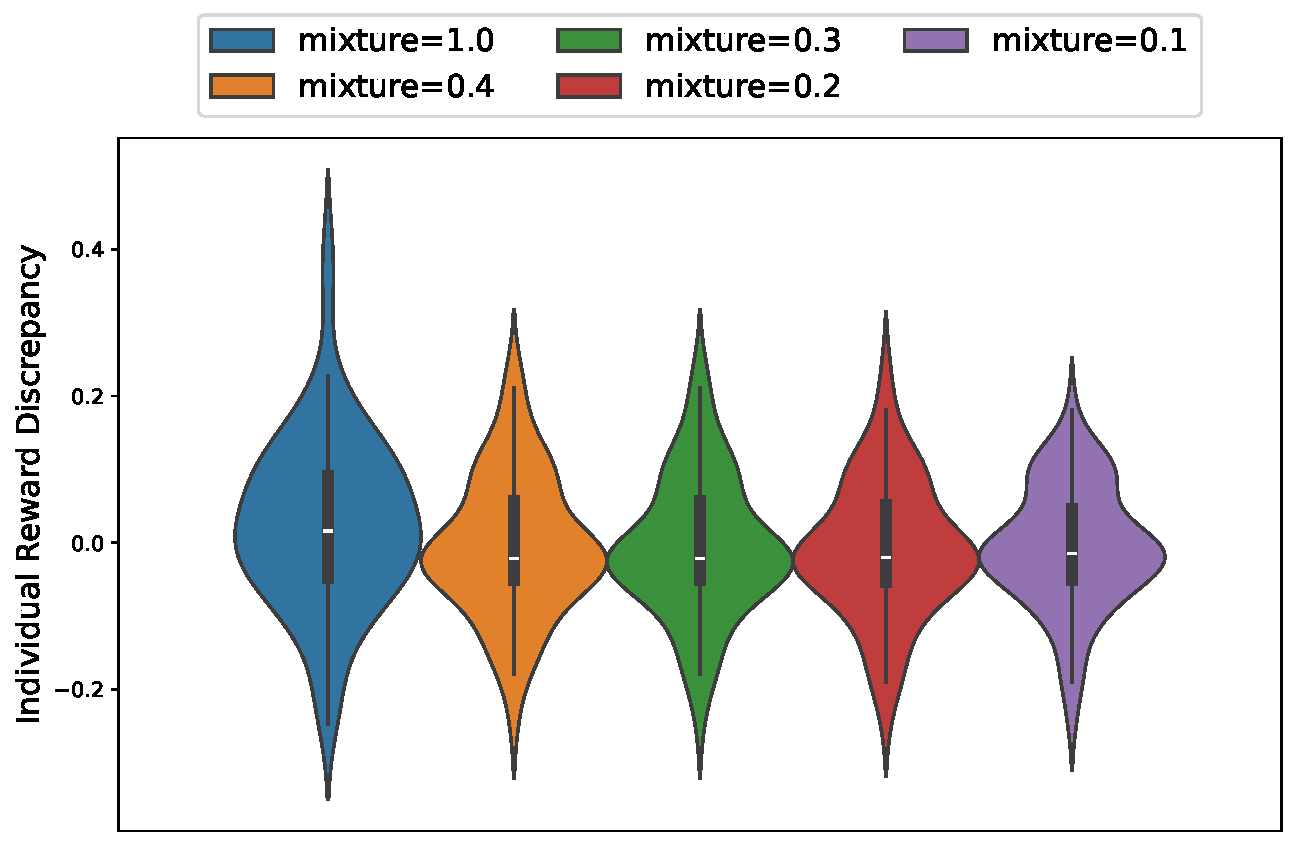
\includegraphics[width=0.6\linewidth]{figs/gap_mixture2.pdf}
    % \vspace{-10pt}
    \caption{
        Distribution of individual reward discrepancies following the Pythia-2.8B model.
    }
    \label{fig_mix}
    % \vspace{-10pt}
\end{figure}
Figure \ref{fig_mix} clearly illustrates that as the mixture ratio increases—that is, the proportion of high gap data rises—the dispersion of the overall dataset broadens. Conversely, a decrease in the mixture ratio, corresponding to an elevated presence of low gap data, results in a more concentrated distribution of reward discrepancy.
% \subsection{$\beta$-DPO and KTO, SPPO}

\begin{figure}[t]
    \vspace{-10pt}
    \centering
    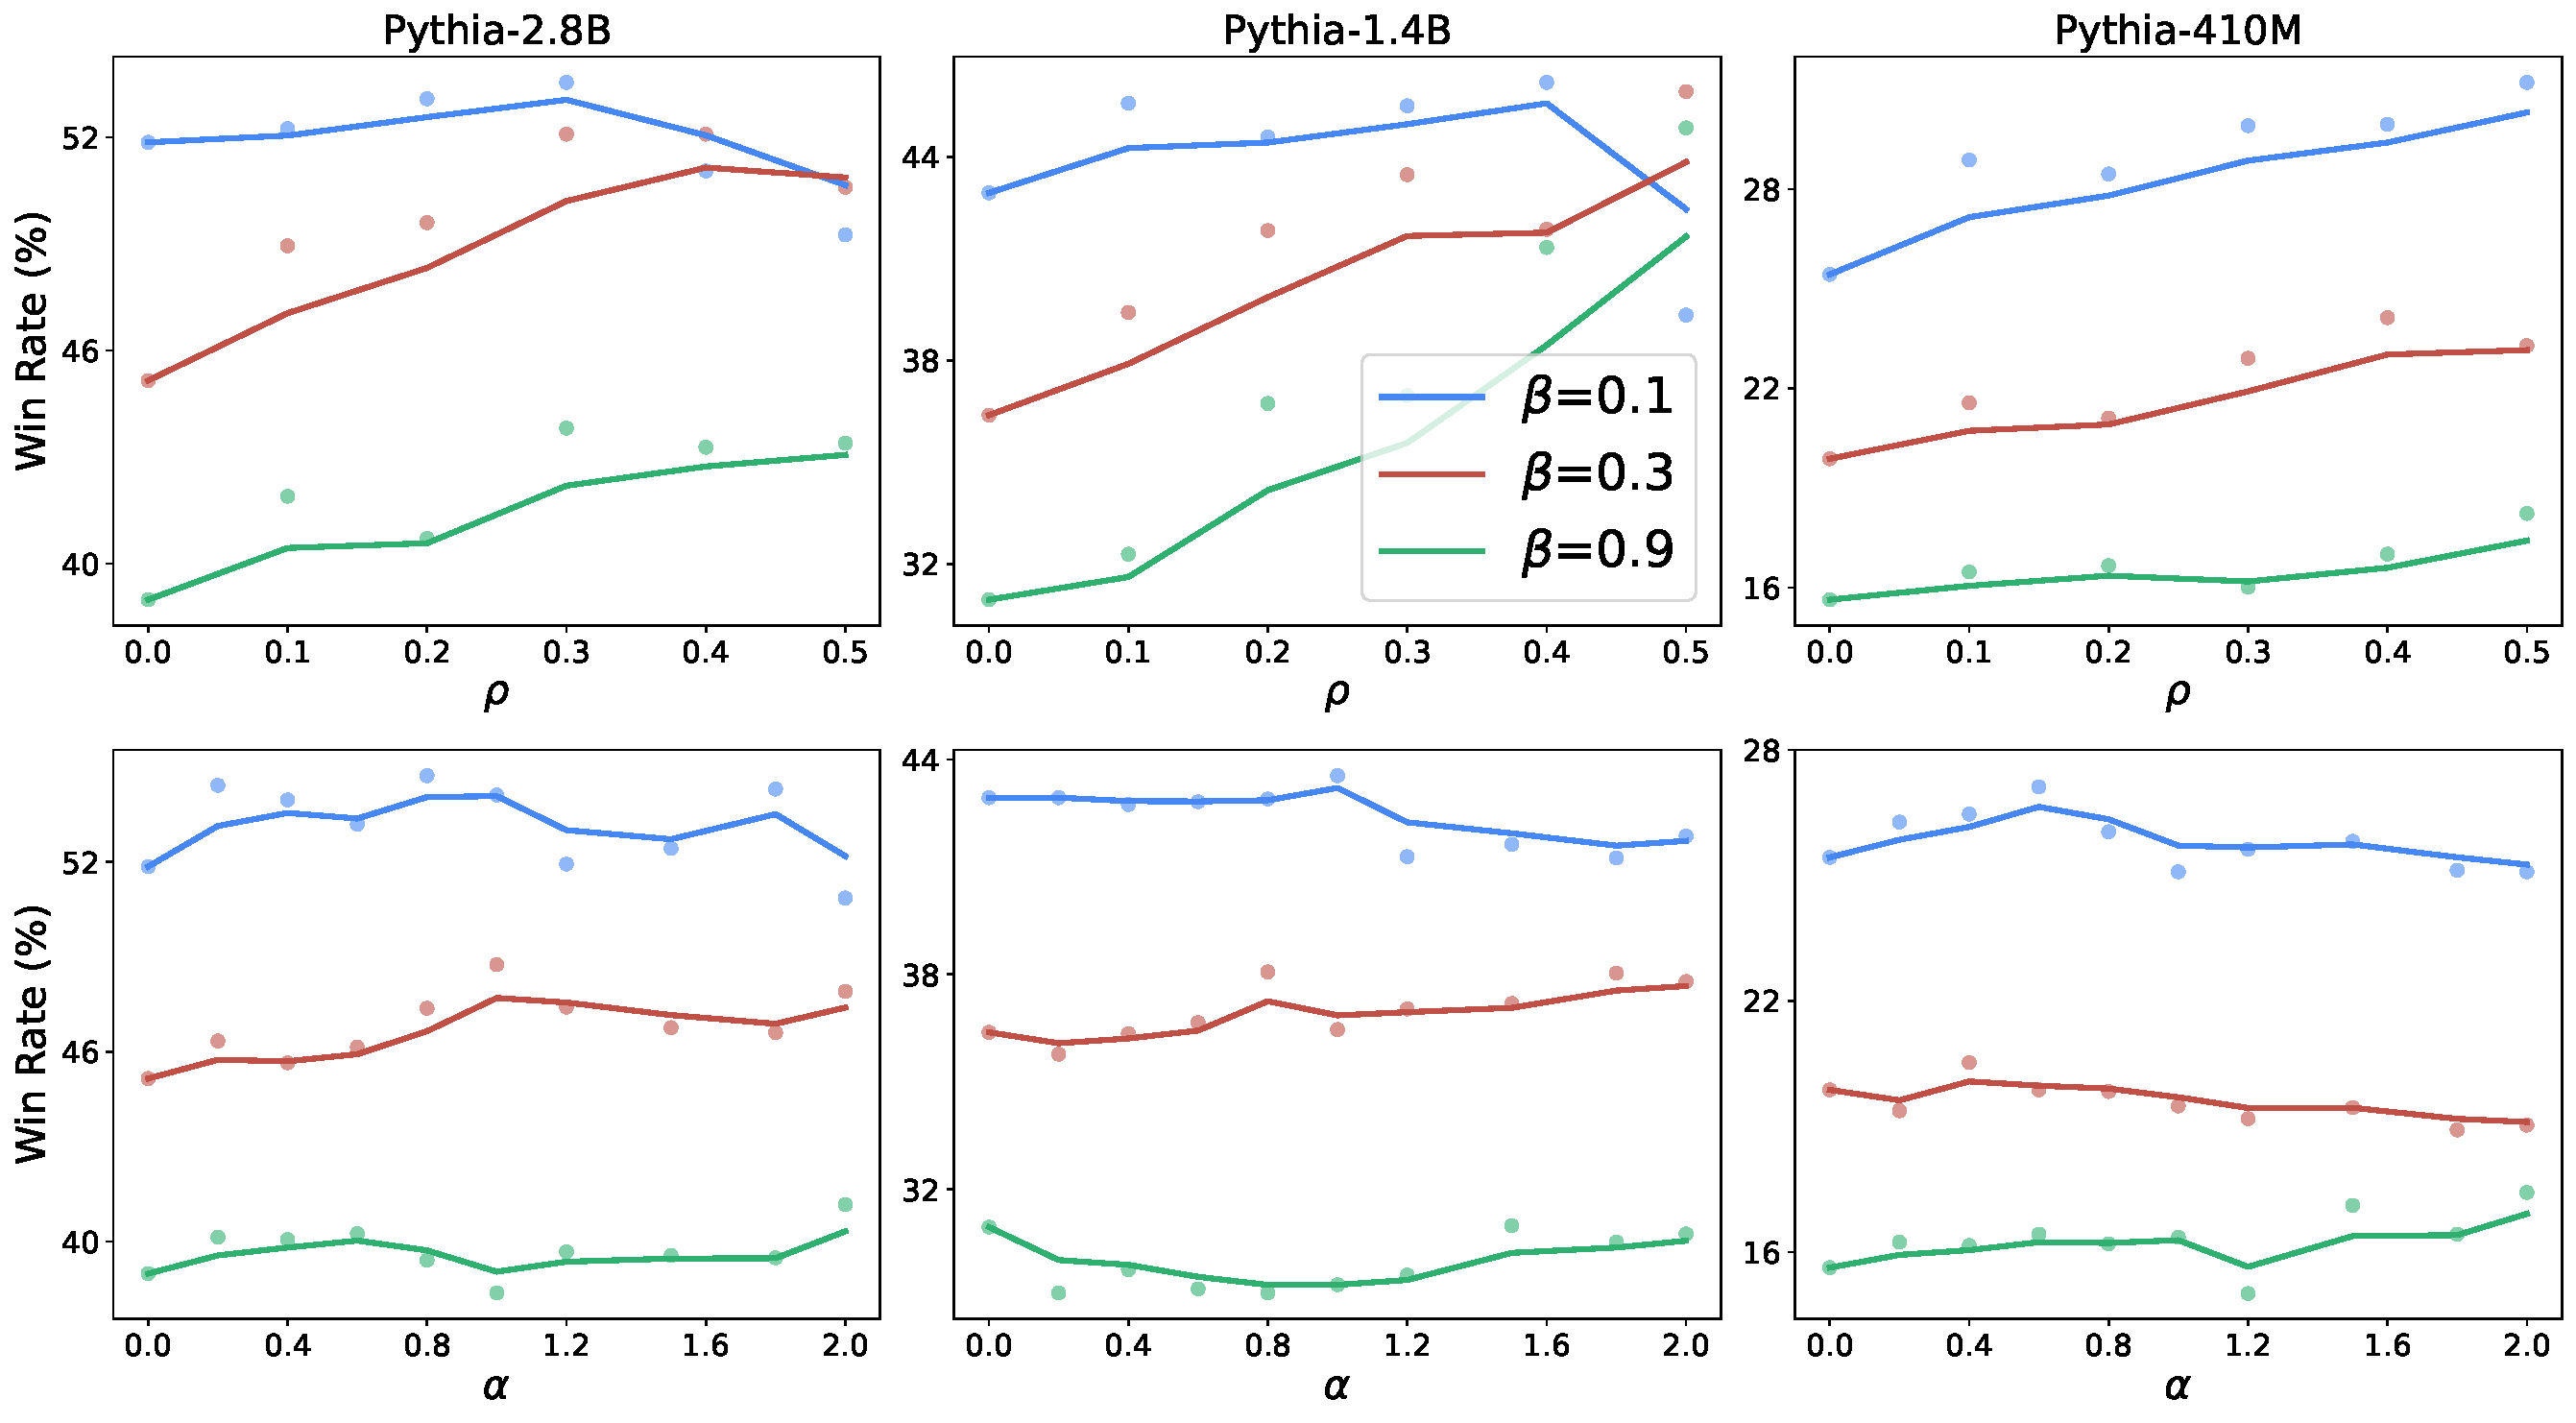
\includegraphics[width=0.8\linewidth]{figs/params_beta_DPO.pdf}
    % \vspace{-10pt}
    \caption{
        Performance comparison across different $\beta$ values and $\rho$ values for three different model sizes (Pythia-2.8B, Pythia-1.4B, and Pythia-410M) on the Anthropic HH dataset using GPT-4 as the evaluator. Each subplot represents the win rate for varying parameters $\beta$ = 0.1, 0.3, and 0.9 with exponential smoothing.
    }
    \label{fig_params}
    \vspace{-10pt}
\end{figure}

\subsection{Hyperparameter Sensitivity}
In this section, we investigate the impact of key hyperparameters in the $\beta$-DPO methodology, using the Anthropic HH dataset and leveraging models such as Pythia-2.8B and GPT-4 for evaluation. Specifically, we examine the influence of varying the hyperparameters $\alpha$ and the filtering ratio $\rho$. The parameter $\alpha$ is explored across a broad spectrum of values including $0.2$, $0.4$, $0.6$, $0.8$, $1.0$, $1.2$, $1.5$, $1.8$, and $2.0$. Concurrently, the filtering ratio $\rho$ is investigated at intervals ranging from $0.1$ to $0.5$, at a granularity of $0.1$. This comprehensive analysis aims to unravel how these hyperparameters affect the performance and outcomes of the $\beta$-DPO process.

\textbf{Static $\beta$ vs. Dynamic $\beta$.}
Our results, as depicted in Figure \ref{fig_params}, reveal that a dynamic $\beta$ (where $\alpha \neq 0$) prevails over a static $\beta$ (where $\alpha = 0$) under an exhaustive range of hyperparameter configurations. 
This outcome aligns seamlessly with our underlying premise: static beta fails to fully leverage a model's potential when confronted with varying data quality within a dataset. Furthermore, our observations highlight an intriguing trend: as $\alpha$ increases, the performance of the $\beta$-DPO model initially improves before declining, typically peaking within the interval of 0.6 to 1.0. 

\textbf{Filtering Ratio $\rho$ Sensitivity.}
As illustrated in the figure \ref{fig_params}, varying model sizes exhibit distinct sensitivities to the parameter $\rho$. Within the context of the Pythia-2.8B model, a $\rho$ value of 0.3 yields optimal performance, whereas for the Pythia-410M model, a $\rho$ value of 0.5 is superior. This can be posited to suggest that smaller models may require more stringent data filtering to perform optimally, whereas larger models possess the increased capacity necessary for learning the most effective strategies. This insight provides a significant directive for future research: the value of $\rho$ should be fine-tuned according to the specific circumstances of the application.


\subsection{The ablation study \wrt $M_0$}
In this work, we employed a moving average updating scheme \cite{mae} for the updating of $M_0$. In order to investigate the superiority of this configuration, we also conducted a comparative experiment involving hyperparameter settings. Specifically, $M_0$ was treated as a constant in the training process, while all other settings remained unchanged. The experimental results are as follows:
\begin{table}[h]
    \centering
    \caption{
    Comparison of win rates across varying $M_0$ in $\beta$-DPO.
    }
    \begin{tabular}{l|l|l|l|l|l|l|l}
        \toprule
        \textbf{$M_0$} & 0 & 1 & 3 & 5& 7& 10 & Moving Average\\
        \midrule
        $\beta$-DPO & $53.35$ & $54.00$ & $53.85$ & $55.61$  &$53.19$ & $56.75$& $57.07$ \\
        \bottomrule
    \end{tabular}
    \label{tab:constant_m0}
\end{table}

As demonstrated in Table \ref{tab:constant_m0}, by tuning $M_0$, we were able to achieve significant performance improvements, which approached the performance level of the moving average updating scheme. This clearly underscores the superiority of the moving average updating scheme. On one hand, it obviates the need for an additional manual search process. On the other hand, it facilitates stable performance enhancements.

\subsection{Our Methods with Explicit Reward Model}
\label{sec:appendix_explicit_rm}
To broaden the application of the $\beta$-DPO strategy for alignment and to address the limitations of DPO's implicit reward model, we incorporated two external reward models (RMs):

\begin{itemize}[leftmargin=*]
    \item We utilized \href{https://huggingface.co/llm-blender/PairRM}{llm-blender/PairRM}~\cite{Jiang2023LLMBlenderEL} to score the chosen and rejected responses, denoted as \(r_{w,\text{PairRM}}, r_{l,\text{PairRM}}\).
    \item We adopted the v0.2 Llama3-Instruct setting \cite{SimPO2024} by employing \href{https://huggingface.co/RLHFlow/ArmoRM-Llama3-8B-v0.1}{{RLHFlow/ArmoRM-Llama3-8B-v0.1}}~\cite{ArmoRM} as the reward model to rank responses, denoted as \(r_{w,\text{ArmoRM}}, r_{l,\text{ArmoRM}}\).
\end{itemize}

{The other algorithmic processes (refer to Appendix Algorithm~\ref{alg:beta-dpo}) remain unchanged, with modifications made only to \(M_{i,\text{PairRM}}=r_{w,\text{PairRM}}^{(i)} - r_{l,\text{PairRM}}^{(i)}\) and \(M_{i,\text{ArmoRM}}=r_{w,\text{ArmoRM}}^{(i)} - r_{l,\text{ArmoRM}}^{(i)}\).} 
For comparison with baselines, we assess our models using one of the most popular open-ended instruction-following benchmarks: AlpacaEval 2.
% We tested the implicit reward model on the state-of-the-art loss function (SimPO \cite{SimPO2024}). 
The detailed results are as follows:

\begin{table}[h]
\centering
\caption{Comparison of different methods on Llama3-Instruct (8B) with explicit reward model}
\begin{tabular}{lcc}
\toprule
\textbf{Method} & \textbf{Llama3-Instruct (8B)} & \textbf{Llama3-Instruct (8B)} \\
\midrule
 & \textbf{LC (\%)} & \textbf{WR (\%)} \\
\midrule
DPO (Implicit RM) & 40.44 & 37.38 \\
$\beta$-DPO (Implicit RM) & \textbf{43.38} & \textbf{38.21} \\
\midrule
SimPO (Implicit RM) & 44.38 & 38.97 \\
$\beta$-SimPO (Implicit RM) & \textbf{46.03} & \textbf{40.18} \\
\midrule
SimPO (PairRM) & 44.70 & 38.98 \\
$\beta$-SimPO (PairRM, Instance-Level) & 43.84 & 38.54 \\
$\beta$-SimPO (PairRM, Batch-Level) & \textbf{45.65} & \textbf{39.76} \\
\midrule
SimPO (ArmoRM) & 53.70 & 47.50 \\
$\beta$-SimPO (ArmoRM, Instance-Level) & 49.05 & 45.47 \\
$\beta$-SimPO (ArmoRM, Batch-Level) & \textbf{54.86} & \textbf{49.66} \\
\bottomrule
\end{tabular}
\label{tab:comparison}
\end{table}

From the results above, we observed the following:

\textbf{The proposed dynamic $\beta$ strategy demonstrates strong generalizability.} Both $\beta$-{D,Sim}PO consistently yield stable performance improvements across implicit and explicit RMs.

\textbf{Batch-level performance is crucial.} In explicit RM settings, batch-level dynamic $\beta$ consistently outperforms instance-level dynamic $\beta$.

\subsection{GPT-4 prompts for computing summarization and dialogue win rates}
\label{app:prompts}
A fundamental element of our experimental framework involves the assessment of win rates facilitated by GPT-4. In this segment, we delineate the prompts employed to ascertain win rates pertinent to our summarization and dialogue-oriented investigations. For the entirety of our experimental endeavors, we utilize GPT-4. It is important to note that the sequence in which summaries or responses are presented is randomized for each evaluation.
% A key component of our experimental setup is GPT-4 win rate judgments. In this section, we include the prompts used to generate win rates for the summarization and dialogue experiments. We use \texttt{gpt-4} for all our experiments. The order of summaries or responses are randomly chosen for every evaluation.
\\[2mm]
\textbf{Summarization GPT-4 win rate prompt.}
\begin{verbatim}
Which of the following summaries does a better job of summarizing the most \
important points in the given forum post?

Post:
<post>

Summary A:
<Summary A>

Summary B:
<Summary B>

FIRST provide a one-sentence comparison of the two summaries, explaining which \
you prefer and why. SECOND, on a new line, state only "A" or "B" to indicate your \ 
choice. Your response should use the format:
Comparison: <one-sentence comparison and explanation>
Preferred: <"A" or "B">
\end{verbatim}

\textbf{Dialogue GPT-4 win rate prompt.}
\begin{verbatim}
For the following query to a chatbot, which response is more helpful?

Query: <the user query>

Response A:
<either the test method or baseline>

Response B:
<the other response>

FIRST provide a one-sentence comparison of the two responses and explain \
which you feel is more helpful. SECOND, on a new line, state only "A" or \
"B" to indicate which response is more helpful. Your response should use \
the format:
Comparison: <one-sentence comparison and explanation>
More helpful: <"A" or "B">
\end{verbatim}

\section{Broader Impacts}
\label{broader_impacts}
This paper presents work whose goal is to advance the field of Machine Learning. There are many potential societal consequences of our work, none of which we feel must be specifically highlighted here.


% Optionally include supplemental material (complete proofs, additional experiments and plots) in appendix.
% All such materials \textbf{SHOULD be included in the main submission.}

%%%%%%%%%%%%%%%%%%%%%%%%%%%%%%%%%%%%%%%%%%%%%%%%%%%%%%%%%%%%

% \newpage
% \clearpage
\section*{NeurIPS Paper Checklist}

% %%% BEGIN INSTRUCTIONS %%%
% % The checklist is designed to encourage best practices for responsible machine learning research, addressing issues of reproducibility, transparency, research ethics, and societal impact. Do not remove the checklist: {\bf The papers not including the checklist will be desk rejected.} The checklist should follow the references and precede the (optional) supplemental material.  The checklist does NOT count towards the page
% % limit. 

% % Please read the checklist guidelines carefully for information on how to answer these questions. For each question in the checklist:
% % \begin{itemize}
% %     \item You should answer \answerYes{}, \answerNo{}, or \answerNA{}.
% %     \item \answerNA{} means either that the question is Not Applicable for that particular paper or the relevant information is Not Available.
% %     \item Please provide a short (1–2 sentence) justification right after your answer (even for NA). 
% %    % \item {\bf The papers not including the checklist will be desk rejected.}
% % \end{itemize}

% % {\bf The checklist answers are an integral part of your paper submission.} They are visible to the reviewers, area chairs, senior area chairs, and ethics reviewers. You will be asked to also include it (after eventual revisions) with the final version of your paper, and its final version will be published with the paper.

% % The reviewers of your paper will be asked to use the checklist as one of the factors in their evaluation. While "\answerYes{}" is generally preferable to "\answerNo{}", it is perfectly acceptable to answer "\answerNo{}" provided a proper justification is given (e.g., "error bars are not reported because it would be too computationally expensive" or "we were unable to find the license for the dataset we used"). In general, answering "\answerNo{}" or "\answerNA{}" is not grounds for rejection. While the questions are phrased in a binary way, we acknowledge that the true answer is often more nuanced, so please just use your best judgment and write a justification to elaborate. All supporting evidence can appear either in the main paper or the supplemental material, provided in appendix. If you answer \answerYes{} to a question, in the justification please point to the section(s) where related material for the question can be found.

% % IMPORTANT, please:
% % \begin{itemize}
% %     \item {\bf Delete this instruction block, but keep the section heading ``NeurIPS paper checklist"},
% %     \item  {\bf Keep the checklist subsection headings, questions/answers and guidelines below.}
% %     \item {\bf Do not modify the questions and only use the provided macros for your answers}.
% % \end{itemize} 
 

% %%% END INSTRUCTIONS %%%


\begin{enumerate}

\item {\bf Claims}
    \item[] Question: Do the main claims made in the abstract and introduction accurately reflect the paper's contributions and scope?
    \item[] Answer: \answerYes{} % Replace by \answerYes{}, \answerNo{}, or \answerNA{}.
    \item[] Justification: see abstract and introduction.
    \item[] Guidelines:
    \begin{itemize}
        \item The answer NA means that the abstract and introduction do not include the claims made in the paper.
        \item The abstract and/or introduction should clearly state the claims made, including the contributions made in the paper and important assumptions and limitations. A No or NA answer to this question will not be perceived well by the reviewers. 
        \item The claims made should match theoretical and experimental results, and reflect how much the results can be expected to generalize to other settings. 
        \item It is fine to include aspirational goals as motivation as long as it is clear that these goals are not attained by the paper. 
    \end{itemize}

\item {\bf Limitations}
    \item[] Question: Does the paper discuss the limitations of the work performed by the authors?
    \item[] Answer: \answerYes{} % Replace by \answerYes{}, \answerNo{}, or \answerNA{}.
    \item[] Justification: see Section \ref{conclusion}.
    \item[] Guidelines:
    \begin{itemize}
        \item The answer NA means that the paper has no limitation while the answer No means that the paper has limitations, but those are not discussed in the paper. 
        \item The authors are encouraged to create a separate "Limitations" section in their paper.
        \item The paper should point out any strong assumptions and how robust the results are to violations of these assumptions (e.g., independence assumptions, noiseless settings, model well-specification, asymptotic approximations only holding locally). The authors should reflect on how these assumptions might be violated in practice and what the implications would be.
        \item The authors should reflect on the scope of the claims made, e.g., if the approach was only tested on a few datasets or with a few runs. In general, empirical results often depend on implicit assumptions, which should be articulated.
        \item The authors should reflect on the factors that influence the performance of the approach. For example, a facial recognition algorithm may perform poorly when image resolution is low or images are taken in low lighting. Or a speech-to-text system might not be used reliably to provide closed captions for online lectures because it fails to handle technical jargon.
        \item The authors should discuss the computational efficiency of the proposed algorithms and how they scale with dataset size.
        \item If applicable, the authors should discuss possible limitations of their approach to address problems of privacy and fairness.
        \item While the authors might fear that complete honesty about limitations might be used by reviewers as grounds for rejection, a worse outcome might be that reviewers discover limitations that aren't acknowledged in the paper. The authors should use their best judgment and recognize that individual actions in favor of transparency play an important role in developing norms that preserve the integrity of the community. Reviewers will be specifically instructed to not penalize honesty concerning limitations.
    \end{itemize}

\item {\bf Theory Assumptions and Proofs}
    \item[] Question: For each theoretical result, does the paper provide the full set of assumptions and a complete (and correct) proof?
    \item[] Answer: \answerNA{} % Replace by \answerYes{}, \answerNo{}, or \answerNA{}.
    \item[] Justification: This work does not include theoretical results.
    \item[] Guidelines:
    \begin{itemize}
        \item The answer NA means that the paper does not include theoretical results. 
        \item All the theorems, formulas, and proofs in the paper should be numbered and cross-referenced.
        \item All assumptions should be clearly stated or referenced in the statement of any theorems.
        \item The proofs can either appear in the main paper or the supplemental material, but if they appear in the supplemental material, the authors are encouraged to provide a short proof sketch to provide intuition. 
        \item Inversely, any informal proof provided in the core of the paper should be complemented by formal proofs provided in appendix or supplemental material.
        \item Theorems and Lemmas that the proof relies upon should be properly referenced. 
    \end{itemize}

    \item {\bf Experimental Result Reproducibility}
    \item[] Question: Does the paper fully disclose all the information needed to reproduce the main experimental results of the paper to the extent that it affects the main claims and/or conclusions of the paper (regardless of whether the code and data are provided or not)?
    \item[] Answer: \answerYes{} % Replace by \answerYes{}, \answerNo{}, or \answerNA{}.
    \item[] Justification: see Appendix \ref{exp_appendix}.
    \item[] Guidelines:
    \begin{itemize}
        \item The answer NA means that the paper does not include experiments.
        \item If the paper includes experiments, a No answer to this question will not be perceived well by the reviewers: Making the paper reproducible is important, regardless of whether the code and data are provided or not.
        \item If the contribution is a dataset and/or model, the authors should describe the steps taken to make their results reproducible or verifiable. 
        \item Depending on the contribution, reproducibility can be accomplished in various ways. For example, if the contribution is a novel architecture, describing the architecture fully might suffice, or if the contribution is a specific model and empirical evaluation, it may be necessary to either make it possible for others to replicate the model with the same dataset, or provide access to the model. In general. releasing code and data is often one good way to accomplish this, but reproducibility can also be provided via detailed instructions for how to replicate the results, access to a hosted model (e.g., in the case of a large language model), releasing of a model checkpoint, or other means that are appropriate to the research performed.
        \item While NeurIPS does not require releasing code, the conference does require all submissions to provide some reasonable avenue for reproducibility, which may depend on the nature of the contribution. For example
        \begin{enumerate}
            \item If the contribution is primarily a new algorithm, the paper should make it clear how to reproduce that algorithm.
            \item If the contribution is primarily a new model architecture, the paper should describe the architecture clearly and fully.
            \item If the contribution is a new model (e.g., a large language model), then there should either be a way to access this model for reproducing the results or a way to reproduce the model (e.g., with an open-source dataset or instructions for how to construct the dataset).
            \item We recognize that reproducibility may be tricky in some cases, in which case authors are welcome to describe the particular way they provide for reproducibility. In the case of closed-source models, it may be that access to the model is limited in some way (e.g., to registered users), but it should be possible for other researchers to have some path to reproducing or verifying the results.
        \end{enumerate}
    \end{itemize}


\item {\bf Open access to data and code}
    \item[] Question: Does the paper provide open access to the data and code, with sufficient instructions to faithfully reproduce the main experimental results, as described in supplemental material?
    \item[] Answer: \answerYes{} % Replace by \answerYes{}, \answerNo{}, or \answerNA{}.
    \item[] Justification: The code is available at \url{https://github.com/junkangwu/beta-DPO}.
    \item[] Guidelines:
    \begin{itemize}
        \item The answer NA means that paper does not include experiments requiring code.
        \item Please see the NeurIPS code and data submission guidelines (\url{https://nips.cc/public/guides/CodeSubmissionPolicy}) for more details.
        \item While we encourage the release of code and data, we understand that this might not be possible, so “No” is an acceptable answer. Papers cannot be rejected simply for not including code, unless this is central to the contribution (e.g., for a new open-source benchmark).
        \item The instructions should contain the exact command and environment needed to run to reproduce the results. See the NeurIPS code and data submission guidelines (\url{https://nips.cc/public/guides/CodeSubmissionPolicy}) for more details.
        \item The authors should provide instructions on data access and preparation, including how to access the raw data, preprocessed data, intermediate data, and generated data, etc.
        \item The authors should provide scripts to reproduce all experimental results for the new proposed method and baselines. If only a subset of experiments are reproducible, they should state which ones are omitted from the script and why.
        \item At submission time, to preserve anonymity, the authors should release anonymized versions (if applicable).
        \item Providing as much information as possible in supplemental material (appended to the paper) is recommended, but including URLs to data and code is permitted.
    \end{itemize}


\item {\bf Experimental Setting/Details}
    \item[] Question: Does the paper specify all the training and test details (e.g., data splits, hyperparameters, how they were chosen, type of optimizer, etc.) necessary to understand the results?
    \item[] Answer: \answerYes{} % Replace by \answerYes{}, \answerNo{}, or \answerNA{}.
    \item[] Justification: see Appendix \ref{exp_appendix}.
    \item[] Guidelines:
    \begin{itemize}
        \item The answer NA means that the paper does not include experiments.
        \item The experimental setting should be presented in the core of the paper to a level of detail that is necessary to appreciate the results and make sense of them.
        \item The full details can be provided either with the code, in appendix, or as supplemental material.
    \end{itemize}

\item {\bf Experiment Statistical Significance}
    \item[] Question: Does the paper report error bars suitably and correctly defined or other appropriate information about the statistical significance of the experiments?
    \item[] Answer: \answerYes{} % Replace by \answerYes{}, \answerNo{}, or \answerNA{}.
    \item[] Justification: The results are accompanied by error bars, confidence intervals, or statistical significance tests, at least for the experiments that support the main claims of the paper.
    \item[] Guidelines:
    \begin{itemize}
        \item The answer NA means that the paper does not include experiments.
        \item The authors should answer "Yes" if the results are accompanied by error bars, confidence intervals, or statistical significance tests, at least for the experiments that support the main claims of the paper.
        \item The factors of variability that the error bars are capturing should be clearly stated (for example, train/test split, initialization, random drawing of some parameter, or overall run with given experimental conditions).
        \item The method for calculating the error bars should be explained (closed form formula, call to a library function, bootstrap, etc.)
        \item The assumptions made should be given (e.g., Normally distributed errors).
        \item It should be clear whether the error bar is the standard deviation or the standard error of the mean.
        \item It is OK to report 1-sigma error bars, but one should state it. The authors should preferably report a 2-sigma error bar than state that they have a 96\% CI, if the hypothesis of Normality of errors is not verified.
        \item For asymmetric distributions, the authors should be careful not to show in tables or figures symmetric error bars that would yield results that are out of range (e.g. negative error rates).
        \item If error bars are reported in tables or plots, The authors should explain in the text how they were calculated and reference the corresponding figures or tables in the text.
    \end{itemize}

\item {\bf Experiments Compute Resources}
    \item[] Question: For each experiment, does the paper provide sufficient information on the computer resources (type of compute workers, memory, time of execution) needed to reproduce the experiments?
    \item[] Answer:  \answerYes{} % Replace by \answerYes{}, \answerNo{}, or \answerNA{}.
    \item[] Justification: We carried out all computational tasks on a suite of four 80GB A100 GPUs.
    \item[] Guidelines:
    \begin{itemize}
        \item The answer NA means that the paper does not include experiments.
        \item The paper should indicate the type of compute workers CPU or GPU, internal cluster, or cloud provider, including relevant memory and storage.
        \item The paper should provide the amount of compute required for each of the individual experimental runs as well as estimate the total compute. 
        \item The paper should disclose whether the full research project required more compute than the experiments reported in the paper (e.g., preliminary or failed experiments that didn't make it into the paper). 
    \end{itemize}
    
\item {\bf Code Of Ethics}
    \item[] Question: Does the research conducted in the paper conform, in every respect, with the NeurIPS Code of Ethics \url{https://neurips.cc/public/EthicsGuidelines}?
    \item[] Answer: \answerYes{} % Replace by \answerYes{}, \answerNo{}, or \answerNA{}.
    \item[] Justification: Our research has been conducted with strict adherence to the NeurIPS Code of Ethics.
    \item[] Guidelines:
    \begin{itemize}
        \item The answer NA means that the authors have not reviewed the NeurIPS Code of Ethics.
        \item If the authors answer No, they should explain the special circumstances that require a deviation from the Code of Ethics.
        \item The authors should make sure to preserve anonymity (e.g., if there is a special consideration due to laws or regulations in their jurisdiction).
    \end{itemize}


\item {\bf Broader Impacts}
    \item[] Question: Does the paper discuss both potential positive societal impacts and negative societal impacts of the work performed?
    \item[] Answer: \answerYes{} % Replace by \answerYes{}, \answerNo{}, or \answerNA{}.
    \item[] Justification: see Appendix \ref{broader_impacts}
    \item[] Guidelines:
    \begin{itemize}
        \item The answer NA means that there is no societal impact of the work performed.
        \item If the authors answer NA or No, they should explain why their work has no societal impact or why the paper does not address societal impact.
        \item Examples of negative societal impacts include potential malicious or unintended uses (e.g., disinformation, generating fake profiles, surveillance), fairness considerations (e.g., deployment of technologies that could make decisions that unfairly impact specific groups), privacy considerations, and security considerations.
        \item The conference expects that many papers will be foundational research and not tied to particular applications, let alone deployments. However, if there is a direct path to any negative applications, the authors should point it out. For example, it is legitimate to point out that an improvement in the quality of generative models could be used to generate deepfakes for disinformation. On the other hand, it is not needed to point out that a generic algorithm for optimizing neural networks could enable people to train models that generate Deepfakes faster.
        \item The authors should consider possible harms that could arise when the technology is being used as intended and functioning correctly, harms that could arise when the technology is being used as intended but gives incorrect results, and harms following from (intentional or unintentional) misuse of the technology.
        \item If there are negative societal impacts, the authors could also discuss possible mitigation strategies (e.g., gated release of models, providing defenses in addition to attacks, mechanisms for monitoring misuse, mechanisms to monitor how a system learns from feedback over time, improving the efficiency and accessibility of ML).
    \end{itemize}
    
\item {\bf Safeguards}
    \item[] Question: Does the paper describe safeguards that have been put in place for responsible release of data or models that have a high risk for misuse (e.g., pretrained language models, image generators, or scraped datasets)?
    \item[] Answer: \answerNA{} % Replace by \answerYes{}, \answerNo{}, or \answerNA{}.
    \item[] Justification: The paper poses no such risks.
    \item[] Guidelines:
    \begin{itemize}
        \item The answer NA means that the paper poses no such risks.
        \item Released models that have a high risk for misuse or dual-use should be released with necessary safeguards to allow for controlled use of the model, for example by requiring that users adhere to usage guidelines or restrictions to access the model or implementing safety filters. 
        \item Datasets that have been scraped from the Internet could pose safety risks. The authors should describe how they avoided releasing unsafe images.
        \item We recognize that providing effective safeguards is challenging, and many papers do not require this, but we encourage authors to take this into account and make a best faith effort.
    \end{itemize}

\item {\bf Licenses for existing assets}
    \item[] Question: Are the creators or original owners of assets (e.g., code, data, models), used in the paper, properly credited and are the license and terms of use explicitly mentioned and properly respected?
    \item[] Answer: \answerNA{} % Replace by \answerYes{}, \answerNo{}, or \answerNA{}.
    \item[] Justification:The answer NA means that the paper does not use existing assets.
    \item[] Guidelines:
    \begin{itemize}
        \item The answer NA means that the paper does not use existing assets.
        \item The authors should cite the original paper that produced the code package or dataset.
        \item The authors should state which version of the asset is used and, if possible, include a URL.
        \item The name of the license (e.g., CC-BY 4.0) should be included for each asset.
        \item For scraped data from a particular source (e.g., website), the copyright and terms of service of that source should be provided.
        \item If assets are released, the license, copyright information, and terms of use in the package should be provided. For popular datasets, \url{paperswithcode.com/datasets} has curated licenses for some datasets. Their licensing guide can help determine the license of a dataset.
        \item For existing datasets that are re-packaged, both the original license and the license of the derived asset (if it has changed) should be provided.
        \item If this information is not available online, the authors are encouraged to reach out to the asset's creators.
    \end{itemize}

\item {\bf New Assets}
    \item[] Question: Are new assets introduced in the paper well documented and is the documentation provided alongside the assets?
    \item[] Answer: \answerNA{} % Replace by \answerYes{}, \answerNo{}, or \answerNA{}.
    \item[] Justification: The answer NA means that the paper does not release new assets.
    \item[] Guidelines:
    \begin{itemize}
        \item The answer NA means that the paper does not release new assets.
        \item Researchers should communicate the details of the dataset/code/model as part of their submissions via structured templates. This includes details about training, license, limitations, etc. 
        \item The paper should discuss whether and how consent was obtained from people whose asset is used.
        \item At submission time, remember to anonymize your assets (if applicable). You can either create an anonymized URL or include an anonymized zip file.
    \end{itemize}

\item {\bf Crowdsourcing and Research with Human Subjects}
    \item[] Question: For crowdsourcing experiments and research with human subjects, does the paper include the full text of instructions given to participants and screenshots, if applicable, as well as details about compensation (if any)? 
    \item[] Answer: \answerNA{} % Replace by \answerYes{}, \answerNo{}, or \answerNA{}.
    \item[] Justification: The paper does not involve crowdsourcing nor research with human subjects.
    \item[] Guidelines:
    \begin{itemize}
        \item The answer NA means that the paper does not involve crowdsourcing nor research with human subjects.
        \item Including this information in the supplemental material is fine, but if the main contribution of the paper involves human subjects, then as much detail as possible should be included in the main paper. 
        \item According to the NeurIPS Code of Ethics, workers involved in data collection, curation, or other labor should be paid at least the minimum wage in the country of the data collector. 
    \end{itemize}

\item {\bf Institutional Review Board (IRB) Approvals or Equivalent for Research with Human Subjects}
    \item[] Question: Does the paper describe potential risks incurred by study participants, whether such risks were disclosed to the subjects, and whether Institutional Review Board (IRB) approvals (or an equivalent approval/review based on the requirements of your country or institution) were obtained?
    \item[] Answer: \answerNA{} % Replace by \answerYes{}, \answerNo{}, or \answerNA{}.
    \item[] Justification: The paper does not involve crowdsourcing nor research with human subjects.
    \item[] Guidelines:
    \begin{itemize}
        \item The answer NA means that the paper does not involve crowdsourcing nor research with human subjects.
        \item Depending on the country in which research is conducted, IRB approval (or equivalent) may be required for any human subjects research. If you obtained IRB approval, you should clearly state this in the paper. 
        \item We recognize that the procedures for this may vary significantly between institutions and locations, and we expect authors to adhere to the NeurIPS Code of Ethics and the guidelines for their institution. 
        \item For initial submissions, do not include any information that would break anonymity (if applicable), such as the institution conducting the review.
    \end{itemize}

\end{enumerate}


\end{document}